\chapter{边界辨识、状态估计与闭环控制}

本章研究有限测温、动态边界未知条件下的一维平板炉温控制。世界模型提供温度场预报，因果边界观测器估计等效换热系数，增广状态滤波器联合校正温度场与边界参数。闭环实验评价状态估计精度、测点布局及后验不确定性对炉温决策的影响。

\section{观测条件与评价安排}

本章沿用一维均匀对称受热平板。炉温动作、材料物性尺度、密度、厚度、时间步长和初始均匀温度均已知；在线需要估计的是温度场以及随时间变化的 $h,\varepsilon$。材料与几何参数不和边界参数同时辨识。测量取自表面、近表面及可选的中心位置，两种布局分别为
\begin{equation}
  \mathcal{S}_4=\{0,0.025,0.975,1\},\qquad
  \mathcal{S}_5=\mathcal{S}_4\cup\{0.5\},
  \label{eq:sensor_layouts}
\end{equation}
其中集合元素为归一化位置 $x/L$。四点布局不测中心温度；五点布局含中心热电偶，适用于仪器化试样或内部测温可用的条件。除专门改变测量条件的实验外，观测噪声均为标准差 \SI{0.5}{\degreeCelsius} 的独立高斯噪声。

开环估计使用预先给定的炉温序列，测量用于更新状态和边界，估计结果不改变炉温。闭环控制根据当前估计重新选择动作，后续温度与测量受到控制策略影响。开环重建精度反映给定动作下的估计能力，闭环效果由反馈轨迹上的误差和控制指标评价。

边界反演采用固定步长数值模型生成的 100 条动态轨迹检查反演误差、确定观测窗口；另行生成的 100 条动态留出轨迹用于评价窗口固定后、由观测器驱动的温度递推。集合滤波使用 BDF 轨迹：10 条用于选择滤波参数，另 90 条用于正式开环估计。边界反演与集合滤波数据的生成器和用途不同，分别统计。

闭环评价包含 10 条未用于滤波校准的 ID 场景，以及参数 OOD 的 10 条探索场景和 40 条独立确认场景；后两组互不重叠，承担不同的研究设计角色。涉及世界模型的比较使用种子 42、7、123 对应的三个已训练模型，在各自评价轨迹上不重新选模或调参。三个种子构成固定模型面板，同一物理场景下的重复运行不作为三个独立工况。直接热平衡反演不依赖网络，其参数误差不按三个模型种子重复计数。

控制器和布局的配对比较以每个场景内三个模型的指标均值为统计量，按场景进行 100000 次 bootstrap。回合成功比例描述执行记录；场景全成功要求三个模型在同一场景下均成功，其 Wilson 区间按独立场景数计算。统计结论以当前模型面板和场景抽样假设为条件，不表示对任意重训练模型或工业炉次的保证。

\section{由历史测温估计等效边界}

在单一表面温度或一维对称两侧温度下，式\eqref{eq:heff}将当前瞬时热流写为 $\Heff$ 与边界温差的乘积。净边界热流的估计可用于恢复这一组合。对表面半控制体应用式\eqref{eq:surface_discrete_balance}，利用相邻时刻的表面和近表面温度，有

\begin{equation}
  \widehat{\Heff}_{n-1}
  =\frac{\widehat{q}_{s,n-1}}{\Tinfty_{n-1}-T_{s,n}}.
  \label{eq:heff_observer}
\end{equation}

$\widehat q_{s,n-1}$ 由半隐式离散热平衡反演，分母使用新时刻表面温度 $T_{s,n}$，与表面离散式一致。状态 $n$ 的测量到达后，观测器得到上一转移的边界估计，并将其用于下一次转移；初始转移采用训练范围中点先验。该时序只需要当前及历史测量。

温度差分容易放大测量噪声，因此对边界平衡式采用后向滑动窗口最小二乘。在生成种子为 20260904 的 100 条动态边界轨迹上扫描窗口后，\SI{0.5}{\degreeCelsius} 噪声条件采用30~s窗口；后续留出评价保持该窗口不变。令窗口分母为 $D_n=\sum_j x_j^2$，其中 $x_j$ 与离散边界温差成正比。当 $D_n\leq10^{-12}$ 时，观测器停用比值更新，返回可行区间中点；其余估计截断至训练边界对应的 $\Heff$ 区间。所报告的反演与留出评价中均未触发低激励回退。

在这组窗口选择轨迹上，无噪声单步反演的 $\Heff$ RMSE 为 \SI{0.002}{\watt\per\square\metre\per\kelvin}；加入 \SI{0.5}{\degreeCelsius} 噪声后，采用 30~s 窗口的误差为 \SI{18.45}{\watt\per\square\metre\per\kelvin}。这两个数值描述反演与窗口选择阶段的表现，不作为独立留出误差。窗口平滑减轻差分噪声，同时引入对边界变化的跟踪滞后，与逆热传导问题的噪声敏感性一致\cite{frankel2007loads,chen2019online}。

生成种子为 20260907 的另100条动态边界留出轨迹用于观测器驱动的温度预测：窗口保持固定，因果观测结果作为世界模型的边界输入，温度场通过模型逐步递推，结果见表\ref{tab:causal_heff_observer}。这组轨迹与上一章表\ref{tab:heff_results}的动态留出集相同，表中均值与样本标准差来自三个模型种子。无噪声时的轨迹误差为 \SI{1.608}{\degreeCelsius}，带噪时增至 \SI{10.018}{\degreeCelsius}。热平衡反演在理想测量下能够支持温度递推，差分噪声则随边界输入传入长期预测。表中残差以各自估计的 $\Heff$ 计算，带噪分支残差较低只表示预测与估计边界较为自洽，不能据此认为其温度预测或真实物理一致性更好。

\begin{table}[H]
  \centering
  \caption{因果边界观测驱动的温度递推，均值$\pm$样本标准差}
  \label{tab:causal_heff_observer}
  \begin{tabular}{lcc}
    \toprule
    测量条件 & 滚动 RMSE/\si{\degreeCelsius} & 估计边界下的残差/\si{\degreeCelsius} \\
    \midrule
    无噪声因果观测 & $1.608\pm0.103$ & $17.37\pm2.78$ \\
    \SI{0.5}{\degreeCelsius} 噪声因果观测 & $10.018\pm0.112$ & $16.40\pm2.76$ \\
    \bottomrule
  \end{tabular}
\end{table}

图\ref{fig:heff_deployment}将因果观测与参考边界输入并列展示。图中的真实 $\Heff$ 由参考表面温度构造，包含额外状态信息，不能用来单独识别参数表示的收益；同信息的自主边界表示比较见表\ref{tab:heff_results}。图\ref{fig:heff_trajectory}取模型种子 42，在联合边界类别内按参考状态条件 $\Heff$ 模型的 RMSE 最接近类别中位数选取轨迹，用于显示边界跟踪和温度误差的对应关系。

\begin{figure}[H]
  \centering
  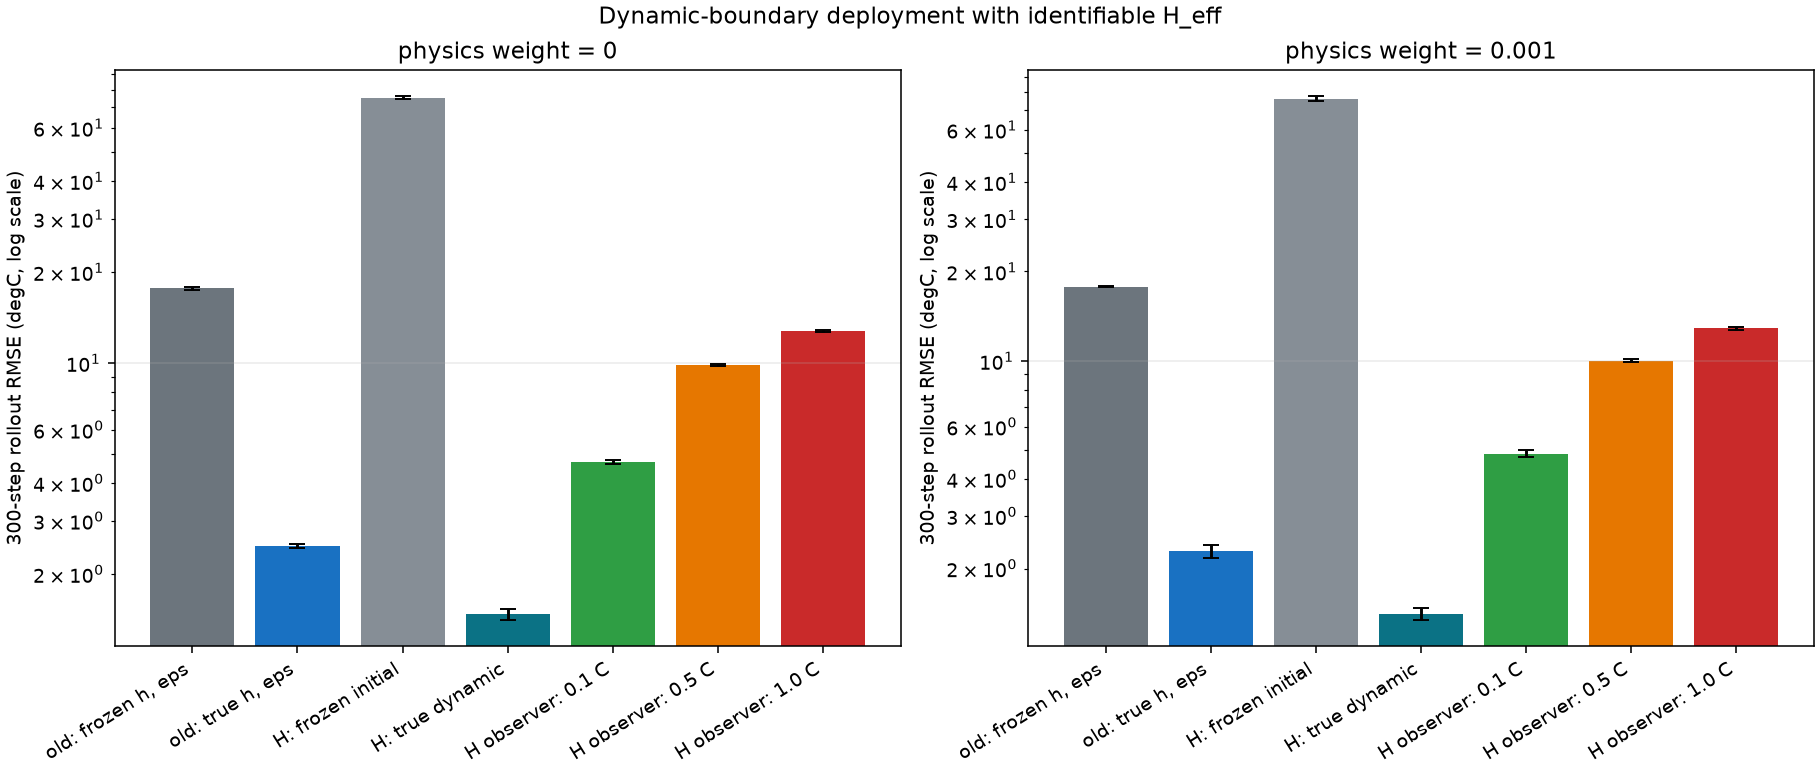
\includegraphics[width=0.96\textwidth]{deployment_comparison.png}
  \caption{参考状态条件边界输入与因果观测方式的比较；同信息自主滚动结果见表\ref{tab:heff_results}}
  \label{fig:heff_deployment}
\end{figure}

\begin{figure}[H]
  \centering
  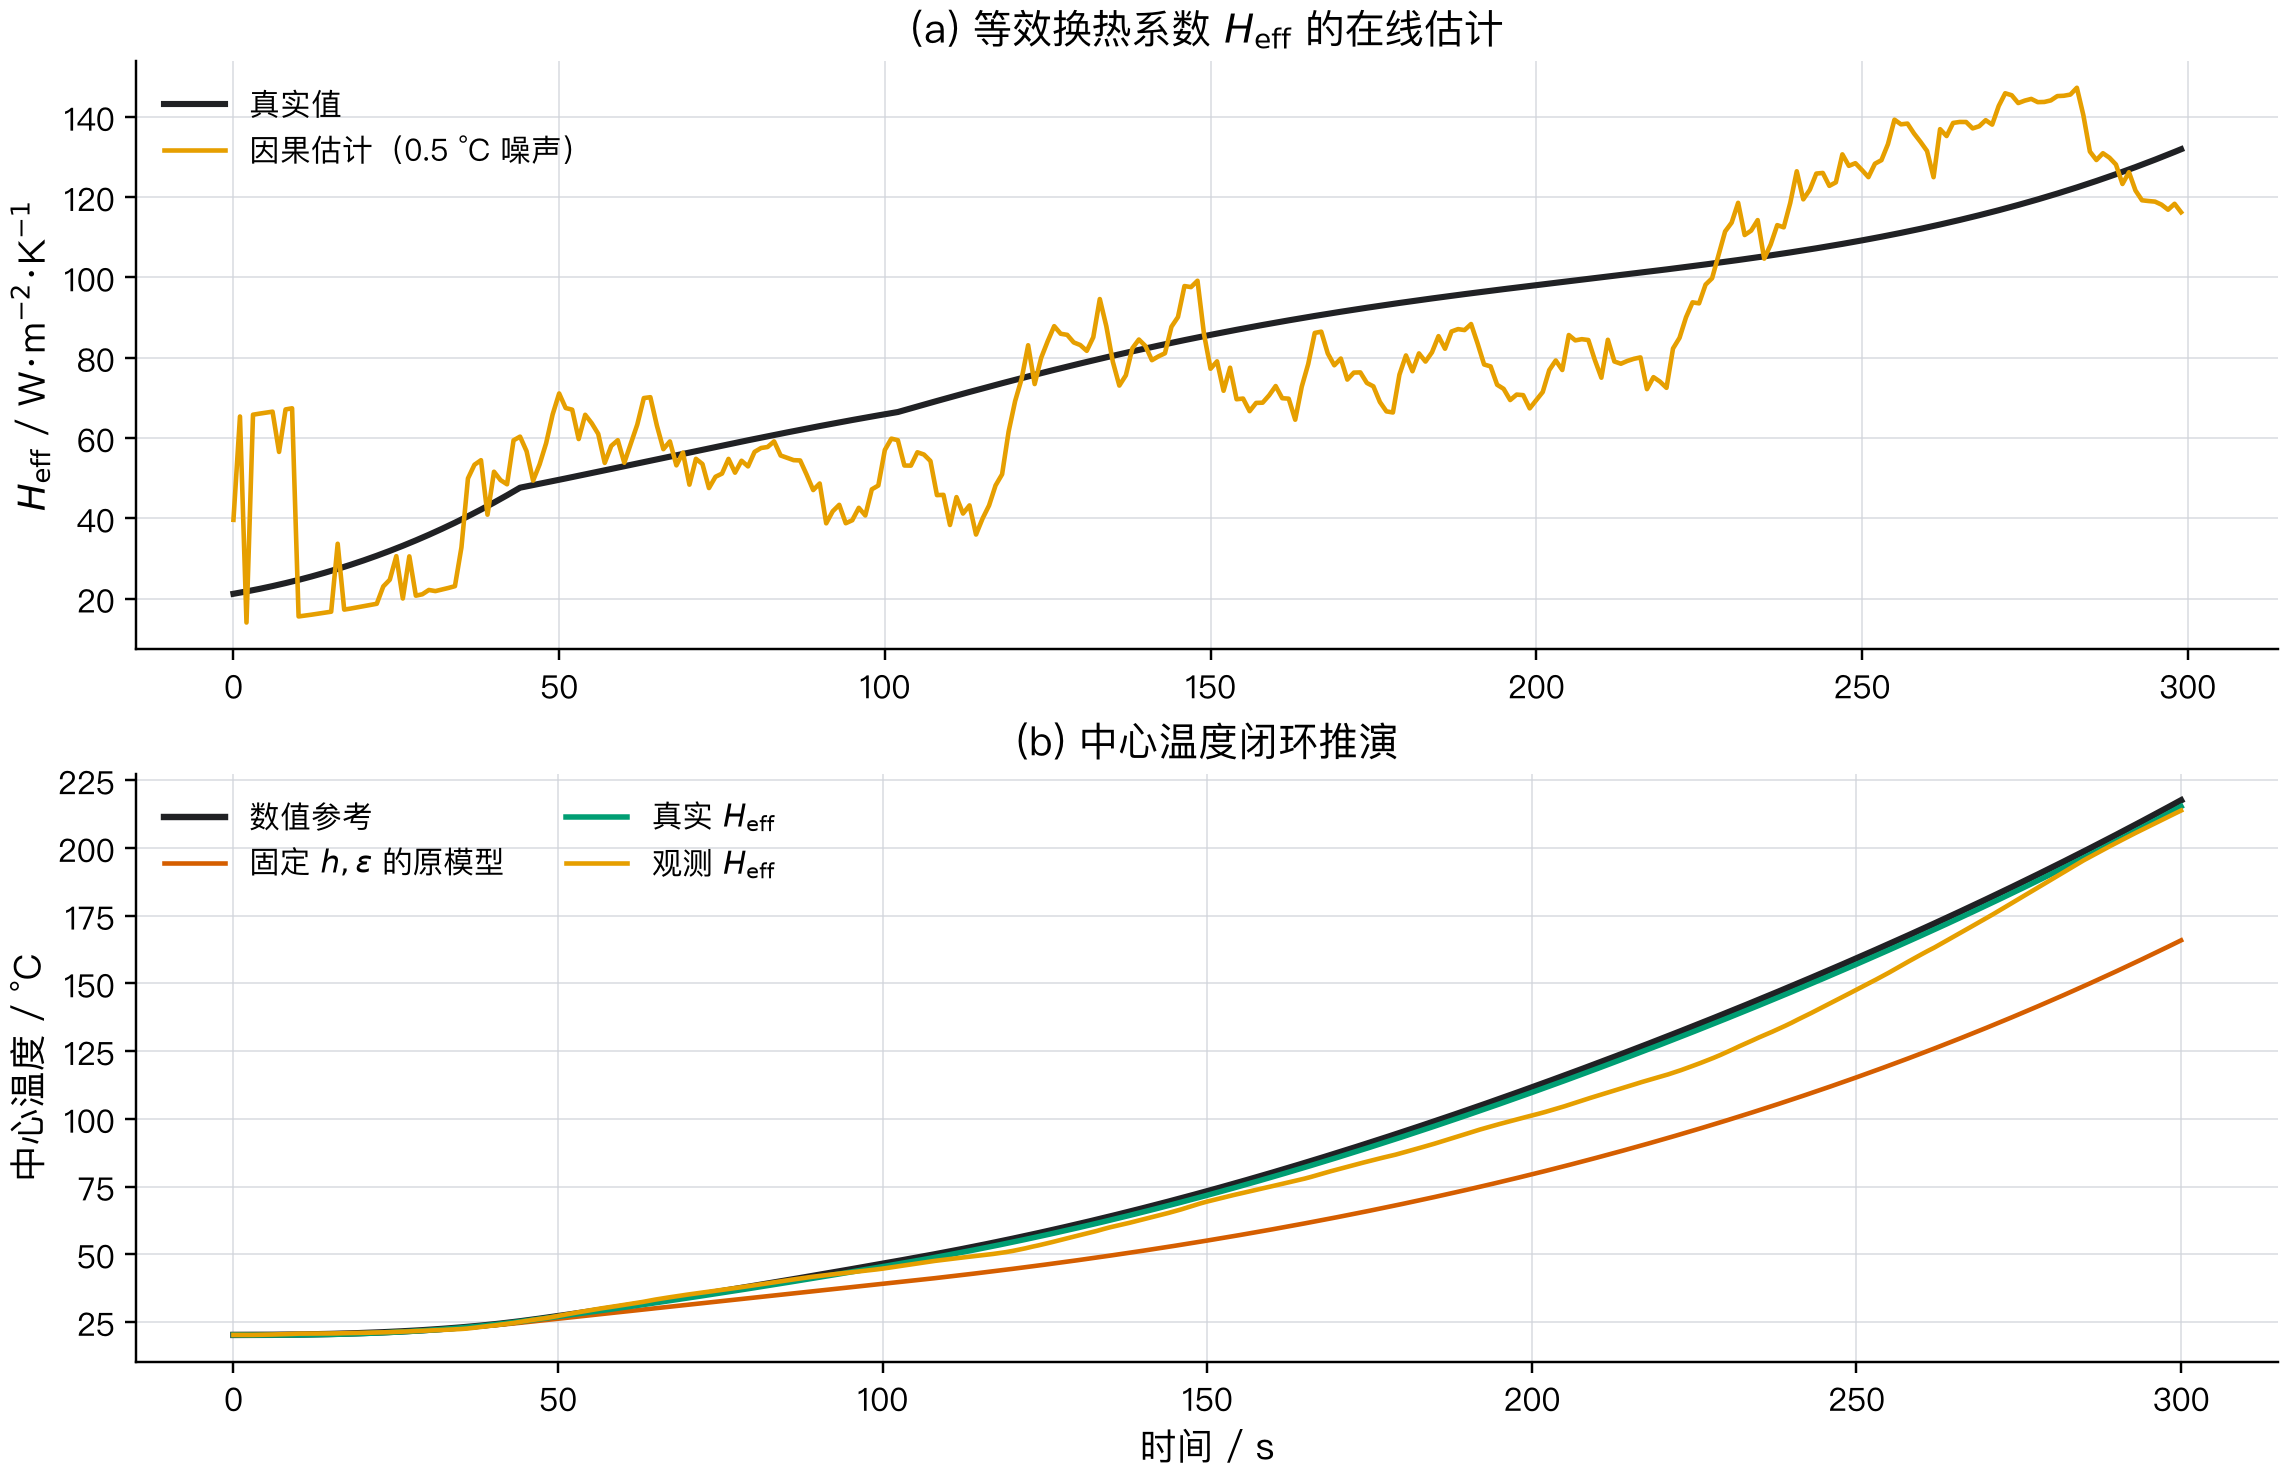
\includegraphics[width=0.96\textwidth]{effective_boundary_trajectory_zh.png}
  \caption{等效换热系数因果观测及给定炉温序列下的递推（真实有效边界采用参考状态条件输入）}
  \label{fig:heff_trajectory}
\end{figure}

图中“闭环推演”指给定炉温序列下的状态递推，不含炉温反馈决策。因果观测能够跟踪边界的主要变化，带噪结果表明仅更新边界输入不足以保持全场精度。集合滤波将稀疏温度测量同时用于温度场和边界参数的校正。

\section{稀疏测温下的温度场重建}

\subsection{增广状态滤波与测点布局}

本文采用 DEnKF，即确定性集合卡尔曼滤波（deterministic ensemble Kalman filter）\cite{evensen2009enkf,oka2020enkf}。温度节点与边界参数组成增广状态
\begin{equation}
  \bm{z}_n=[T_1^n,\ldots,T_{41}^n,h_n,\varepsilon_n]^{\mathsf T}.
\end{equation}
64 个集合成员分别经过世界模型预报，并通过式\eqref{eq:heff}生成各自的有效边界输入。测量更新利用温度状态、边界参数与测点温度之间的样本交叉协方差进行联合校正；温度场同时保持本研究的中心面对称条件。配置见表\ref{tab:enkf_config}。这里对 $h,\varepsilon$ 的分解受到动态先验、参数支持域和历史观测共同约束，不表示从单次瞬时热流就能唯一识别两者。

\begin{table}[H]
  \centering
  \caption{增广状态集合滤波配置}
  \label{tab:enkf_config}
  \begin{tabular}{lc@{\qquad}lc}
    \toprule
    参数 & 数值 & 参数 & 数值 \\
    \midrule
    集合规模 & 64 & 测温噪声标准差 & \SI{0.5}{\degreeCelsius} \\
    初始温度场标准差 & \SI{0.25}{\degreeCelsius} & 温度状态过程噪声 & \SI{0.03}{\degreeCelsius} \\
    $h$ 初始先验 & $35\pm12$~\si{\watt\per\square\metre\per\kelvin} & $h$ 过程噪声 & \SI{1.0}{\watt\per\square\metre\per\kelvin} \\
    $\varepsilon$ 初始先验 & $0.775\pm0.070$ & $\varepsilon$ 过程噪声 & 0.004 \\
    集合膨胀系数 & 1.01 & 局部化半径 & 8 个节点 \\
    \bottomrule
  \end{tabular}
\end{table}

区间由集合成员的 5\% 和 95\% 分位数构成。未测节点覆盖率统计除初始状态外、参考温度落入该区间的节点--时刻比例；$h,\varepsilon$ 的覆盖率按全部参数时刻统计。90 条开环评价轨迹与三个模型共形成 270 条模型--场景记录，测点布局比较见表\ref{tab:sensor_layout}。

\begin{table}[H]
  \centering
  \caption{稀疏测点布局的温度场重建结果，RMSE 单位：\si{\degreeCelsius}}
  \label{tab:sensor_layout}
  \small
  \resizebox{\textwidth}{!}{%
  \begin{tabular}{lcccc}
    \toprule
    传感器布局 & \shortstack{全场\\RMSE} & \shortstack{未测节点\\RMSE} & \shortstack{中心\\RMSE} & \shortstack{未测节点\\90\% 覆盖率} \\
    \midrule
    无中心测点的近表面 4 点 & 2.022 & 2.128 & 2.854 & $81.5\%$ \\
    含中心热电偶的理想 5 点 & 1.008 & 1.073 & 0.231 & $90.8\%$ \\
    \bottomrule
  \end{tabular}}
\end{table}

四点布局的未测节点 RMSE 为 \SI{2.128}{\degreeCelsius}，中心 RMSE 为 \SI{2.854}{\degreeCelsius}。五点布局的相应误差更低，但 \SI{0.231}{\degreeCelsius} 的中心 RMSE 包含直接中心测量的校正效果，不能解释为仅由表面温度推断心部的精度。两种布局各自未测节点集合也不同。有限测点下的重建能力必须连同测点位置解释，这与已有温度场重建研究的结论一致\cite{liu2022reconstruction}。图\ref{fig:assimilation}给出五点条件下的温度场与边界同化结果。

\begin{figure}[H]
  \centering
  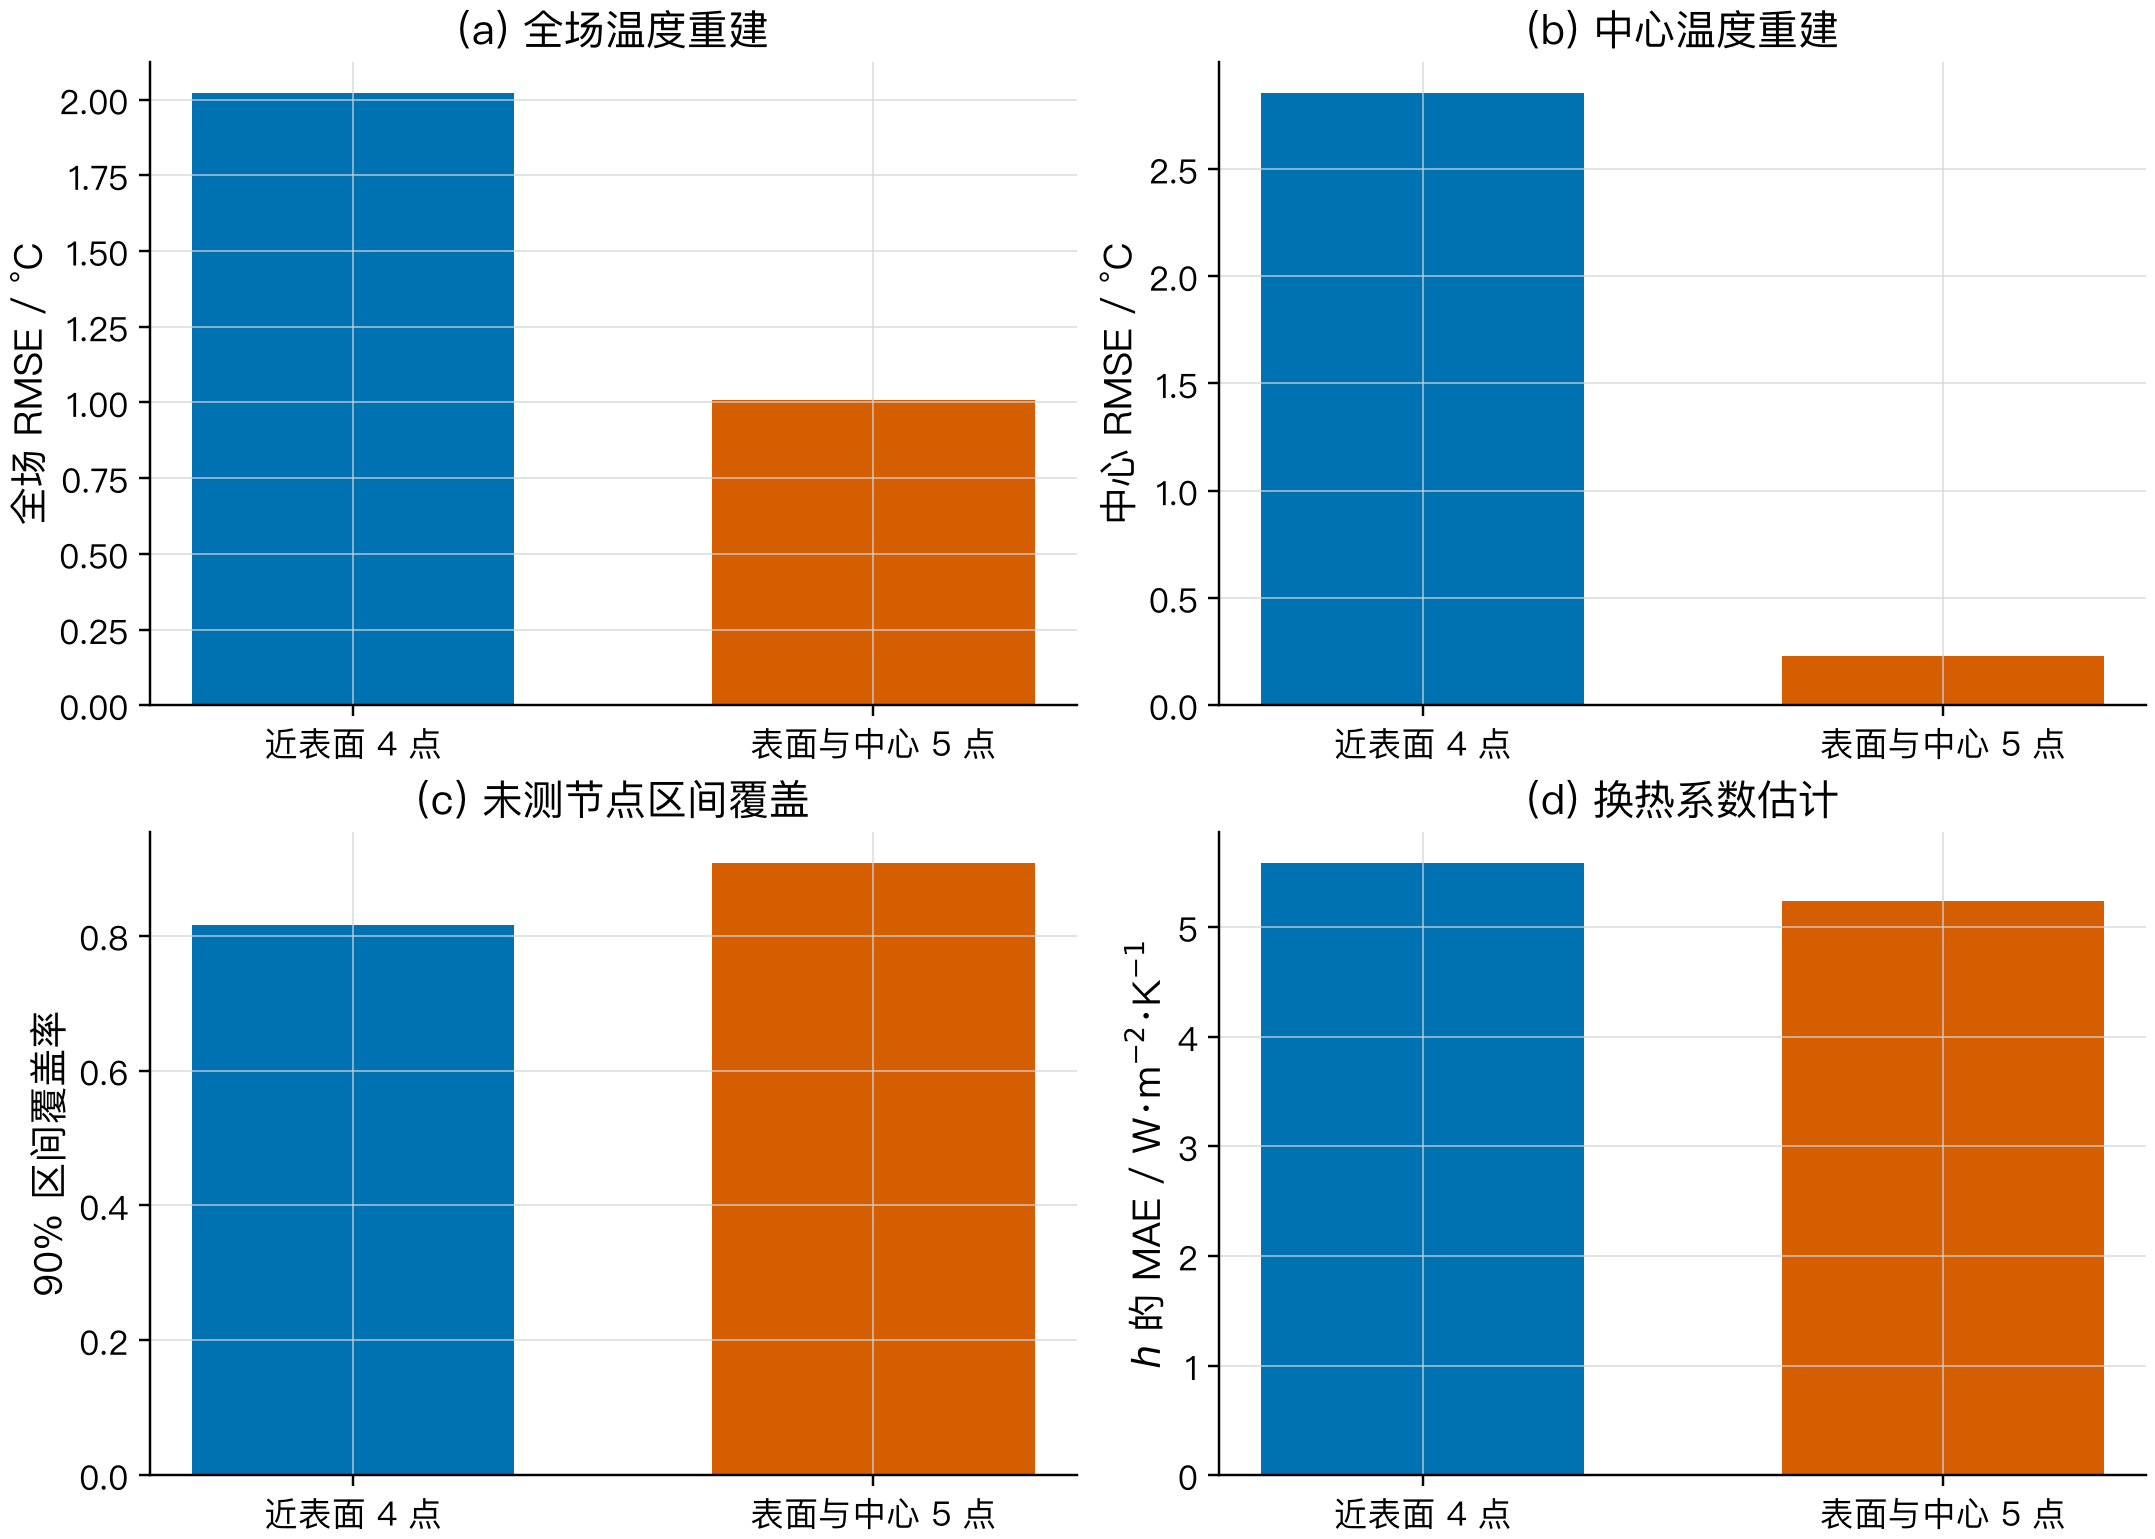
\includegraphics[width=0.96\textwidth]{open_loop_assimilation.png}
  \caption{五点测温条件下的温度场与边界参数同化结果}
  \label{fig:assimilation}
\end{figure}

参数支持域同样影响估计。在五点参数 OOD 评价中，沿用训练范围截断后验时，全场 RMSE 为 \SI{5.247}{\degreeCelsius}。将支持域扩展为 $h\in[5,80]$~\si{\watt\per\square\metre\per\kelvin}、$\varepsilon\in[0.45,0.98]$，同时把初始先验标准差从 12、0.070 分别增至 15、0.100 后，全场 RMSE 降至 \SI{2.813}{\degreeCelsius}，中心 RMSE 为 \SI{0.290}{\degreeCelsius}，两种参数的 90\% 区间覆盖率分别为 $79.9\%$ 和 $76.5\%$。该比较支持扩大支持域与先验不确定性的整体配置，未单独识别其中某一项的贡献。

\subsection{测量噪声与传感器响应}

测量噪声与响应迟滞在四点布局下分别评价：改变噪声标准差，并用一阶响应生成滞后测温。每个条件包含 90 条 BDF 轨迹和三个模型，滤波器统一按瞬时测量处理。结果见表\ref{tab:sensor_robustness}与图\ref{fig:sensor_robustness}。

\begin{table}[H]
  \centering
  \caption{近表面四点测温的噪声与响应滞后结果}
  \label{tab:sensor_robustness}
  \resizebox{\textwidth}{!}{%
  \begin{tabular}{lccc}
    \toprule
    测量条件 & 未测节点 RMSE/\si{\degreeCelsius} & 中心 RMSE/\si{\degreeCelsius} & 90\% 覆盖率 \\
    \midrule
    噪声 \SI{0.2}{\degreeCelsius} & 2.297 & 2.985 & $73.9\%$ \\
    噪声 \SI{0.5}{\degreeCelsius} & 2.128 & 2.854 & $81.5\%$ \\
    噪声 \SI{1.0}{\degreeCelsius} & 2.100 & 2.853 & $86.0\%$ \\
    \SI{2}{\second} 响应时间常数，噪声 \SI{0.5}{\degreeCelsius} & 2.691 & 3.433 & $65.2\%$ \\
    \SI{5}{\second} 响应时间常数，噪声 \SI{0.5}{\degreeCelsius} & 4.894 & 5.501 & $34.4\%$ \\
    \bottomrule
  \end{tabular}}
\end{table}

噪声标准差从 \SI{0.2}{\degreeCelsius} 增至 \SI{1.0}{\degreeCelsius} 时，RMSE 没有明显恶化，区间覆盖率随之上升。观测协方差按实际噪声同步设置，噪声增大也降低了滤波器对局部测量的权重，结果不能解释为增加噪声具有一般收益。忽略响应迟滞时，时间常数为 \SI{5}{\second} 的未测节点 RMSE 增至 \SI{4.894}{\degreeCelsius}，覆盖率降至 $34.4\%$。误差增加与覆盖率下降对应观测方程和测量动态的不匹配。

\begin{figure}[H]
  \centering
  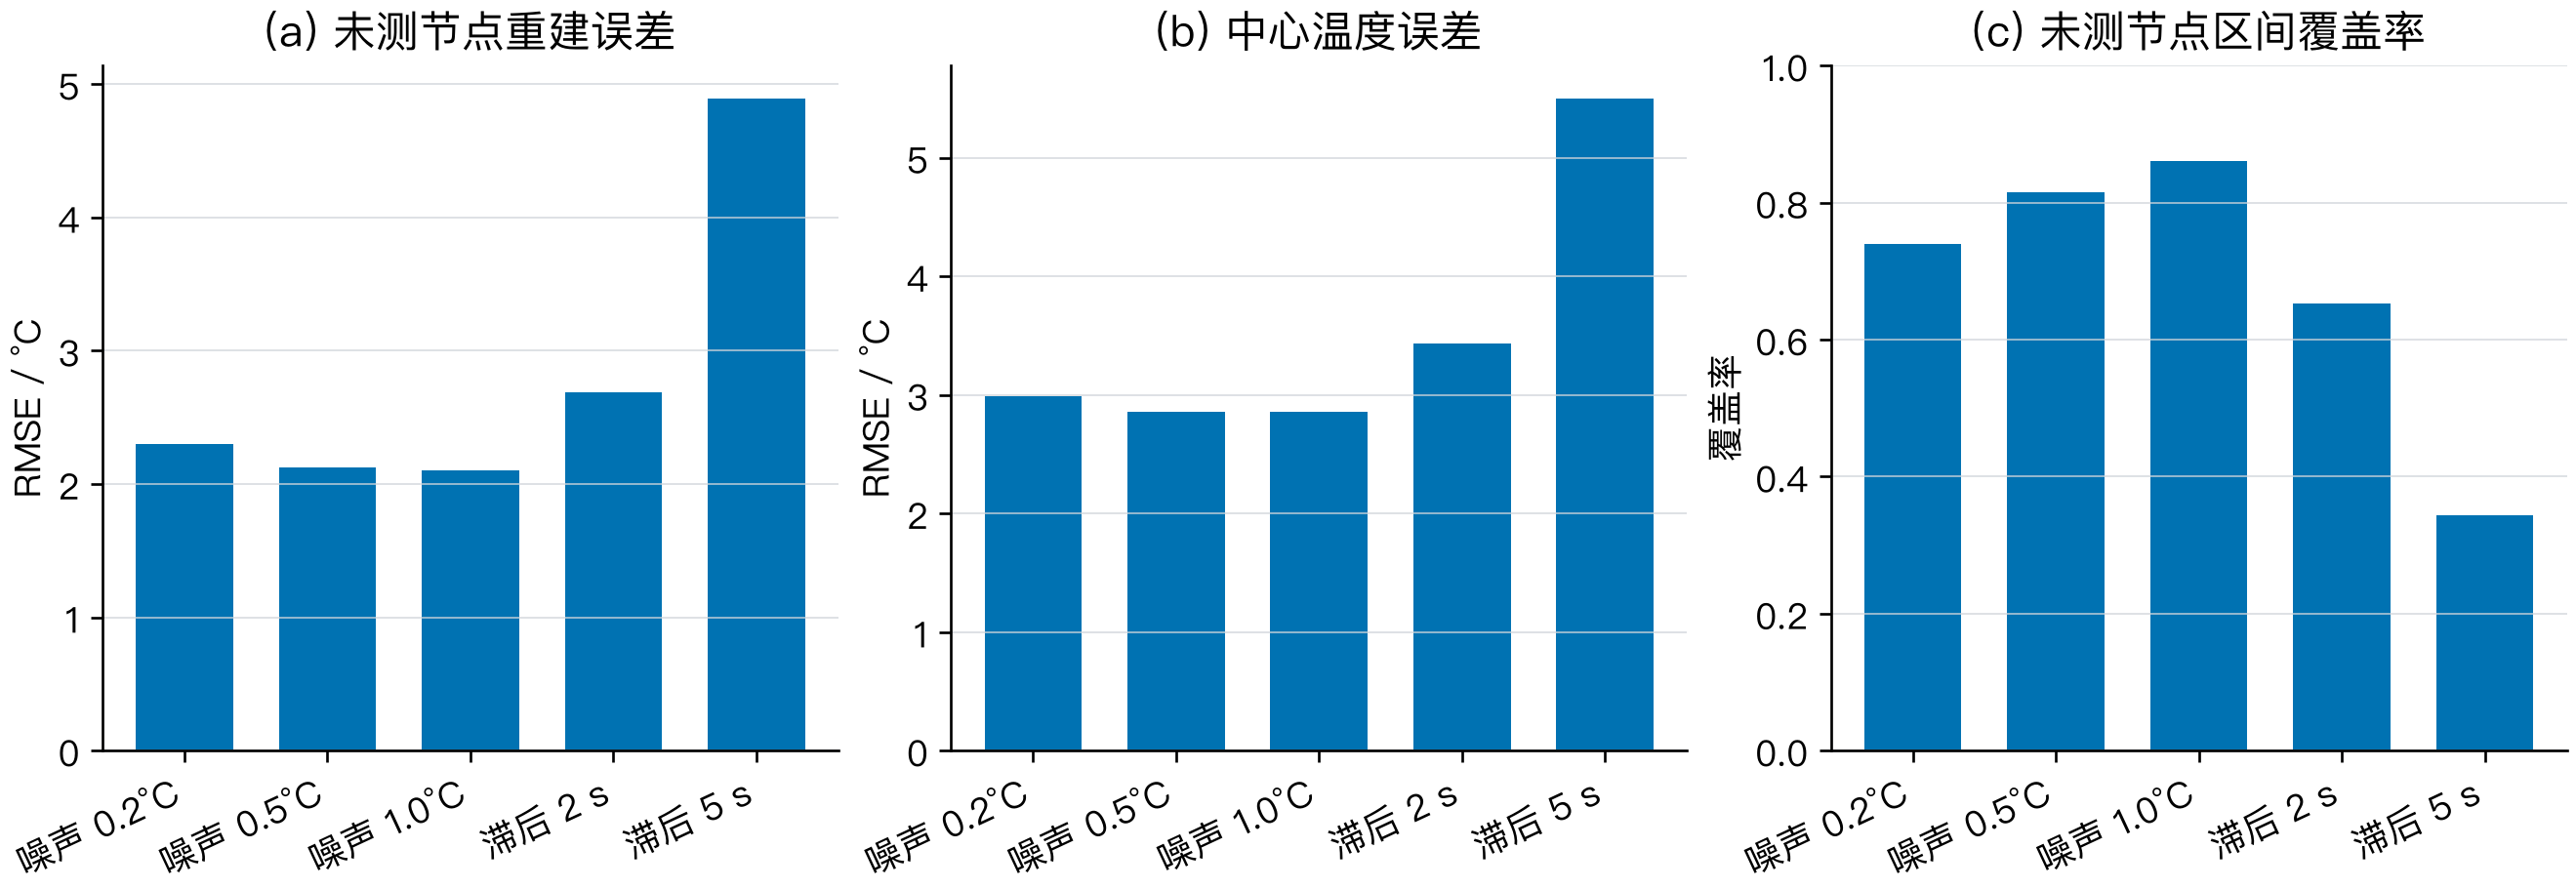
\includegraphics[width=0.96\textwidth]{sensor_robustness.png}
  \caption{近表面稀疏测温对随机噪声与传感器响应滞后的鲁棒性}
  \label{fig:sensor_robustness}
\end{figure}

为匹配观测动态，在增广状态中增加四个传感器响应状态 $r_{j,n}$：

\begin{equation}
  r_{j,n+1}=\alpha r_{j,n}+(1-\alpha)T_{i_j,n+1},\qquad
  y_{j,n+1}=r_{j,n+1}+v_{j,n+1},\qquad
  \alpha=\exp(-\Delta t/\tau_s).
  \label{eq:sensor_response}
\end{equation}

其中 $i_j$ 为测点节点，$\tau_s$ 为响应时间常数，$v_{j,n}$ 的标准差为 \SI{0.5}{\degreeCelsius}。递推采用采样区间内温度取右端值的分段常数近似，初始传感器温度与工件平衡，与迟滞试验的生成方式一致。预报阶段以推演得到的工件温度更新响应状态；同化阶段以响应状态预测测量，并通过交叉协方差校正温度场与边界。该过程只使用已经到达的测量。

真实时间常数预先固定为 2 s 和 5 s。校准使用集合滤波的10条独立校准轨迹及已知测点真温度，在 0--8 s、间隔 0.1 s 的候选网格上最小化响应预测与带噪测量的平方误差，分别选中 2.0 s 和 5.0 s 后固定。该仪器化标定以独立温度参照为前提，未检验从未知工件温度同时识别传感器和边界的能力。

瞬时观测与响应状态两种滤波器共用模型、测量序列、初始随机数及过程噪声；集合规模、局部化、膨胀和边界先验保持一致。两种响应条件、两种滤波器、90 条评价轨迹与三个模型共形成 1080 条记录，其中瞬时观测分支的 540 条记录与前述迟滞试验逐项一致。表\ref{tab:sensor_response}给出留出结果。

\begin{table}[H]
  \centering
  \caption{响应状态补偿的留出轨迹结果，每行 90 条轨迹、三个模型种子}
  \label{tab:sensor_response}
  \small
  \begin{tabular}{clrrrr}
    \toprule
    $\tau_s$/s & 观测模型 & \shortstack{未测节点\\RMSE/°C} & \shortstack{中心\\RMSE/°C} & \shortstack{90\% 区间\\覆盖率} & \shortstack{区间平均\\宽度/°C} \\
    \midrule
    2 & 瞬时观测 & 2.691 & 3.433 & $65.2\%$ & 5.382 \\
    2 & 响应状态 & 2.147 & 2.881 & $82.5\%$ & 5.567 \\
    5 & 瞬时观测 & 4.894 & 5.501 & $34.4\%$ & 5.384 \\
    5 & 响应状态 & 2.178 & 2.932 & $84.2\%$ & 5.931 \\
    \bottomrule
  \end{tabular}
\end{table}

轨迹配对结果显示，2 s 条件的未测节点 RMSE 差为 \SI{-0.544}{\degreeCelsius}，95\% 区间为 $[-0.692,-0.394]$~\si{\degreeCelsius}。5 s 条件的配对差为 \SI{-2.716}{\degreeCelsius}，区间为 $[-3.095,-2.342]$~\si{\degreeCelsius}。5 s 条件的误差降低 $55.5\%$，覆盖率提高约 49.8 个百分点，区间平均宽度增加 \SI{0.546}{\degreeCelsius}。响应状态补偿同时降低点估计误差、提高区间覆盖率，支持其减轻迟滞偏差的作用。

\begin{figure}[H]
  \centering
  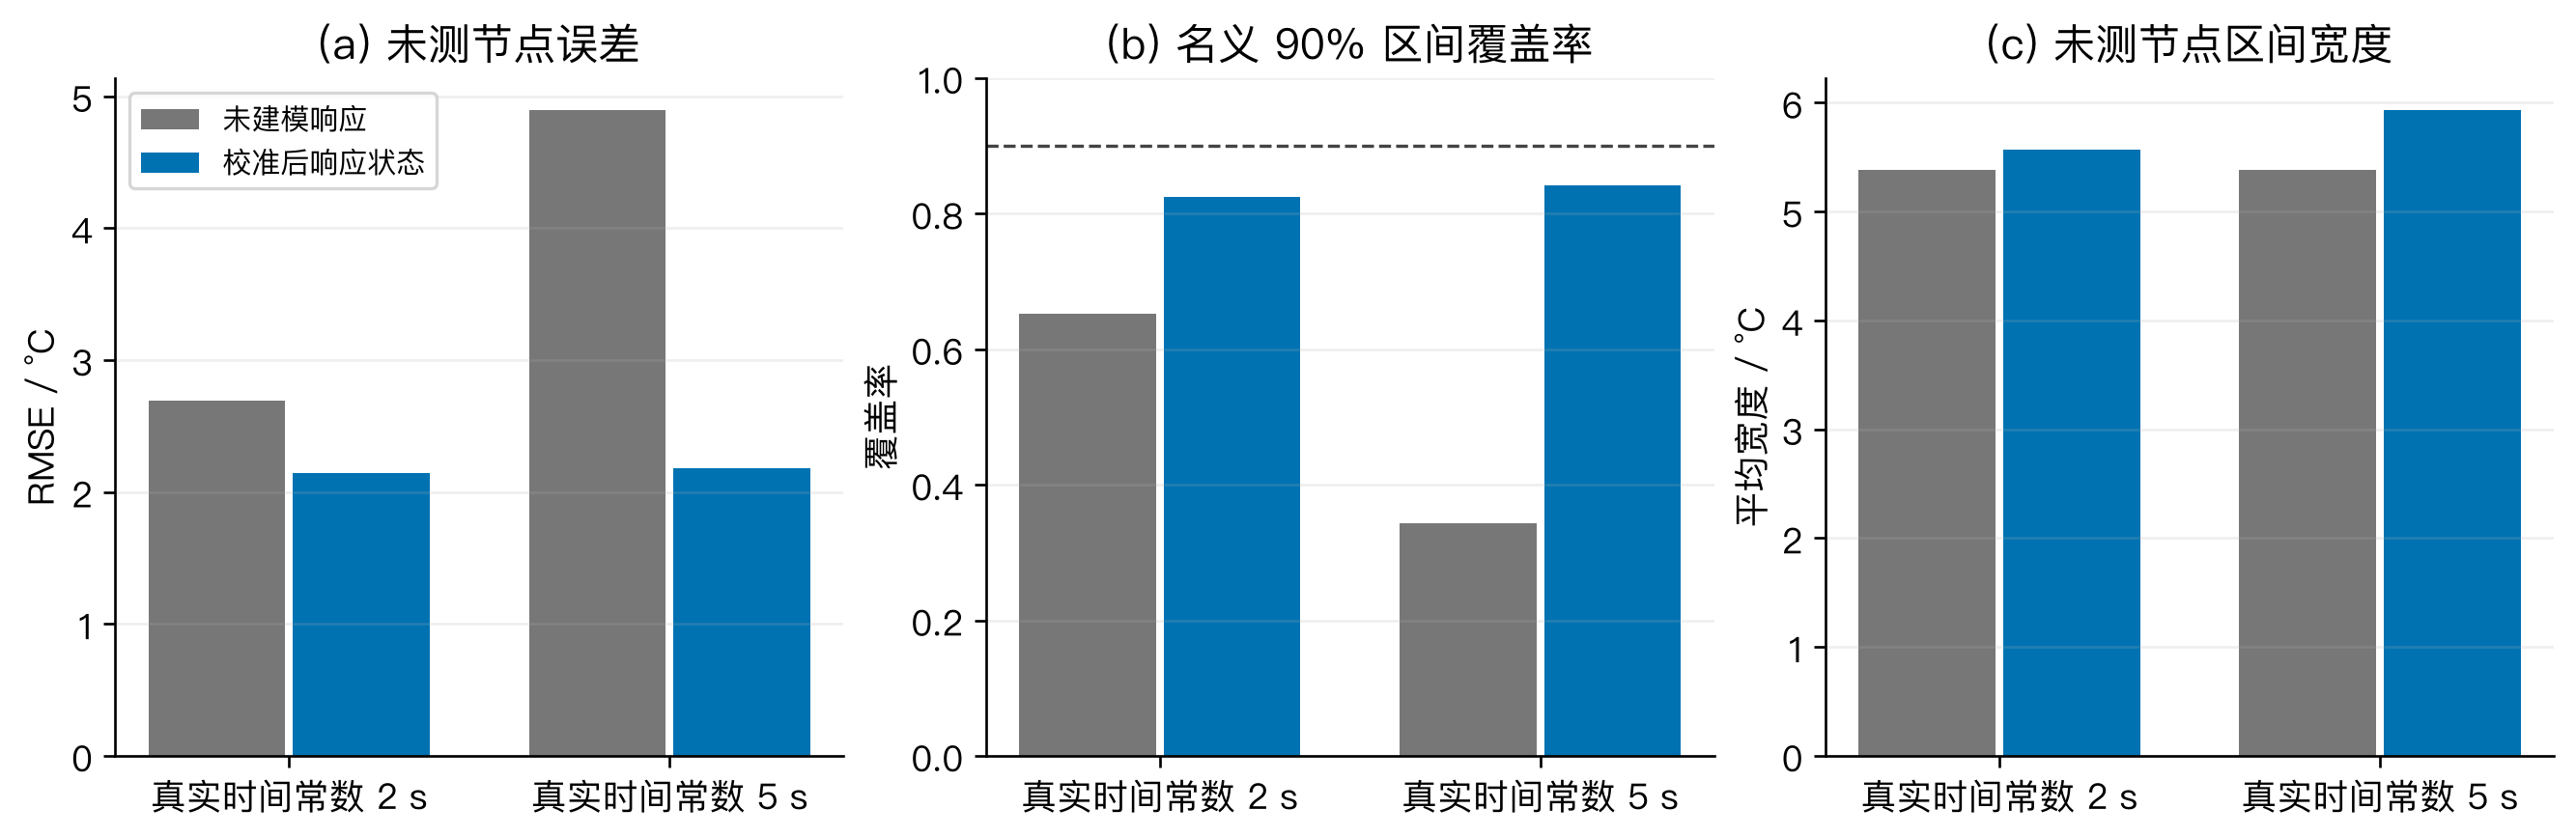
\includegraphics[width=0.98\textwidth]{sensor_response.png}
  \caption{独立校准的传感器响应状态对误差及区间质量的影响}
  \label{fig:sensor_response}
\end{figure}

补偿后的未测节点误差接近无滞后基准，但 $82.5\%$--$84.2\%$ 的覆盖率仍低于名义 $90\%$。证据限于合成一阶传感器及独立响应标定可用的开环估计，未覆盖时间常数漂移、测点响应差异或真实校准误差。后续闭环实验使用无响应滞后的合成测量，不能把本节的补偿收益直接归入闭环控制结果。

\section{共同闭环策略与信息对照}

控制器每 20~s 根据当前状态选择一次炉温，在总长 300~s 的任务内跟踪 \SI{350}{\degreeCelsius} 的中心目标。候选炉温为 $\{300,400,500,600,700,800,900,950\}$~\si{\degreeCelsius}。每个候选值在剩余预测时域内保持常数，选定后只执行首个 20~s 区间，再利用新的观测更新状态。该控制器采用常值尾部的单移动阻塞 MPC，搜索变量仅为当前炉温值。目标温度和约束用于检验控制链路，不构成完整的 C45 工业热处理制度。

所有对照使用相同的候选动作目标函数：

\begin{equation}
  J=|T_c^{\mathrm{end}}-T^*|
  +0.25\Delta T^{\mathrm{end}}
  +5\max(0,T_s^{\max}-T_{\mathrm{lim}})
  +5E+0.01V,
  \label{eq:control_objective}
\end{equation}

其中 $\Delta T^{\mathrm{end}}=\max_i T_i^{\mathrm{end}}-\min_i T_i^{\mathrm{end}}$，$T_s^{\max}$ 为预测时域内两侧表面的最高温度，$E=(a-20)/(950-20)$ 为归一化炉温项，$V=|a-a_{\mathrm{prev}}|$ 为本次动作变化。表面温度上限 $T_{\mathrm{lim}}$ 在 ID 任务中为 \SI{550}{\degreeCelsius}，在参数 OOD 压力测试中收紧至 \SI{360}{\degreeCelsius}。超温通过代价惩罚处理，并非优化器强制满足的硬约束；归一化炉温项也不等同于实测能耗。

执行完回合后，以实际温度和动作轨迹计算综合目标

\begin{equation}
  J_{\mathrm{ep}}=|T_c^{\mathrm{end}}-T^*|
  +0.25\Delta T^{\mathrm{end}}+5O+5\overline{E}+0.01V_{\mathrm{ep}},
  \label{eq:episode_control_objective}
\end{equation}

其中 $O=\max(0,\max_{n,s}T_{s,n}-T_{\mathrm{lim}})$，$\overline E$ 为 300 个执行时刻的归一化炉温均值，$V_{\mathrm{ep}}=|a_1-300|+\sum_{k=2}^{N_{\mathrm{dec}}}|a_k-a_{k-1}|$ 为决策序列总变差，$N_{\mathrm{dec}}$ 为决策次数。表中的“中心误差”指终点中心绝对误差，“平均超温”指各回合峰值超温量 $O$ 的平均。终点中心误差不超过 \SI{10}{\degreeCelsius} 且 $O=0$ 时，记为成功回合\cite{rawlings2017mpc}。

四种控制器使用不同的状态与边界信息。完整状态与真实边界控制器获得完整真实温度场和剩余时域的真实 $h,\varepsilon$ 序列；稀疏状态与真实边界控制器使用滤波温度场估计，未来边界仍已知。两者构成区分状态误差和边界不确定性影响的理想信息对照。后验均值控制由当前测量驱动，使用滤波均值，并将当前 $h,\varepsilon$ 估计保持至预测末端；风险分位控制使用 16 个后验成员，按候选代价的 90\% 分位选择动作\cite{moehle2021risk}。

这两种后验控制在规划中都不读取未来真实边界，也不传播未来边界过程噪声。风险分位数因此描述当前后验、固定参数预测假设下的代价差异，不能解释为表面超温概率保证。候选炉温改变时，辐射基函数也随之改变，必须用每个成员的 $h,\varepsilon$ 和预测表面温度重新计算 $\Heff$。单一的当前 $\Heff$ 只约束既定状态与动作的瞬时热流；其离散转移充分性限于第三章所述冻结旧状态系数的格式，不能替代候选动作下的参数后验。

\section{ID 跟踪与测点布局的闭环影响}

\subsection{理想信息基准与五点测温}

世界模型与 BDF 的动作搜索在 10 条动态边界场景上比较。两者使用相同的代价、候选动作与预测时域，每次决策均获得各自网格上的完整真实状态和全部未来真实边界，仅更换预测动力学及对应网格。世界模型的三个种子共运行 30 个回合，终点中心误差为 \SI{2.096}{\degreeCelsius}，30/30 个回合成功，对应 10/10 个场景全成功及 $[72.2\%,100\%]$ 的95\% Wilson 区间。BDF 搜索在 10/10 个场景成功，终点误差为 \SI{2.120}{\degreeCelsius}。

这一理想条件下，每回合候选规划时间分别为 \SI{0.099}{\second} 与 \SI{6.258}{\second}，比值为 63.4。该计时只对应完整真实状态和未来边界已知的候选动作搜索，任务与表\ref{tab:fair_timing}的完整轨迹推演不同，不能合并为统一速度结论。若仅将边界输入改为 \SI{0.5}{\degreeCelsius} 噪声下的因果观测、仍保留完整真实状态，终点误差为 \SI{3.906}{\degreeCelsius}，成功回合为28/30，场景全成功为9/10，95\%区间为 $[59.6\%,98.2\%]$。这一对照尚未包含由稀疏测温恢复全场的误差。

\begin{figure}[H]
  \centering
  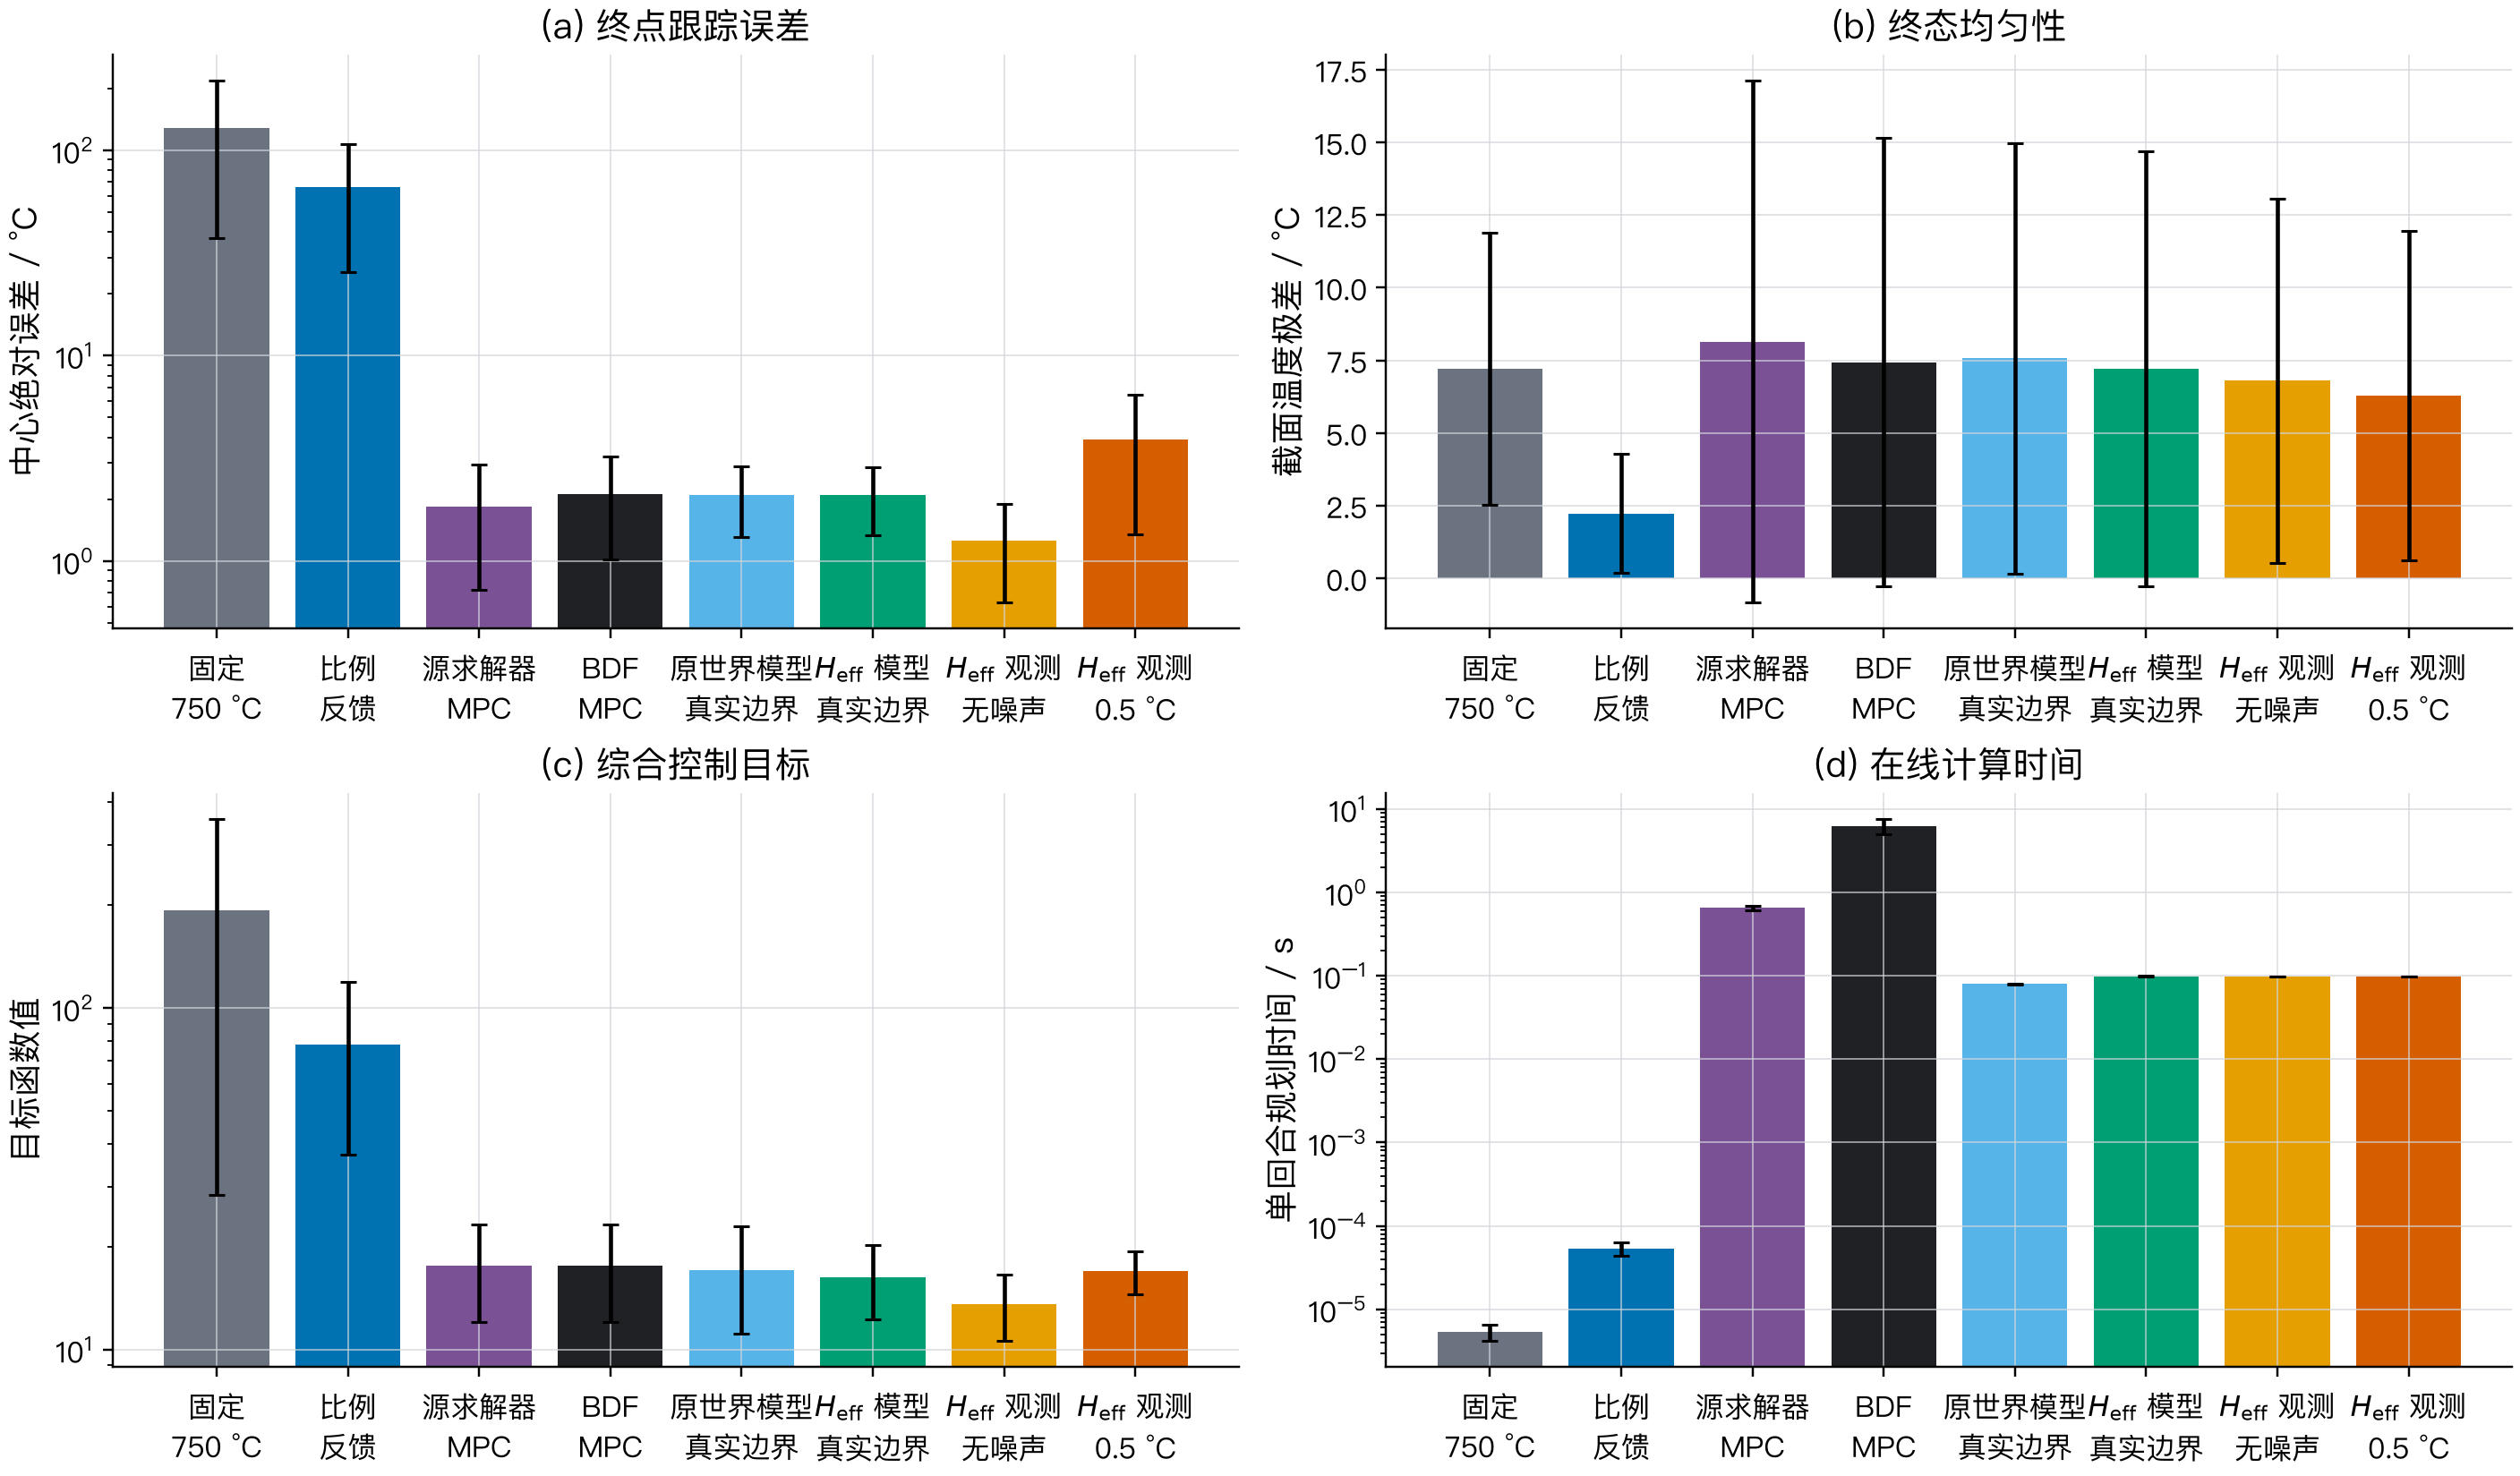
\includegraphics[width=0.96\textwidth]{closed_loop_control_summary.png}
  \caption{完整状态输入下的动态边界滚动动作搜索；真实边界分支获得全部未来边界}
  \label{fig:closed_loop}
\end{figure}

图\ref{fig:closed_loop_trajectory}取模型种子 42 和联合边界轨迹 12。固定炉温产生目标过冲，比例反馈在后段升温不足，BDF 与世界模型动作搜索的终点温度均接近目标。这一代表性轨迹用于说明动作选择的作用，整体判断以场景统计为准。

\begin{figure}[H]
  \centering
  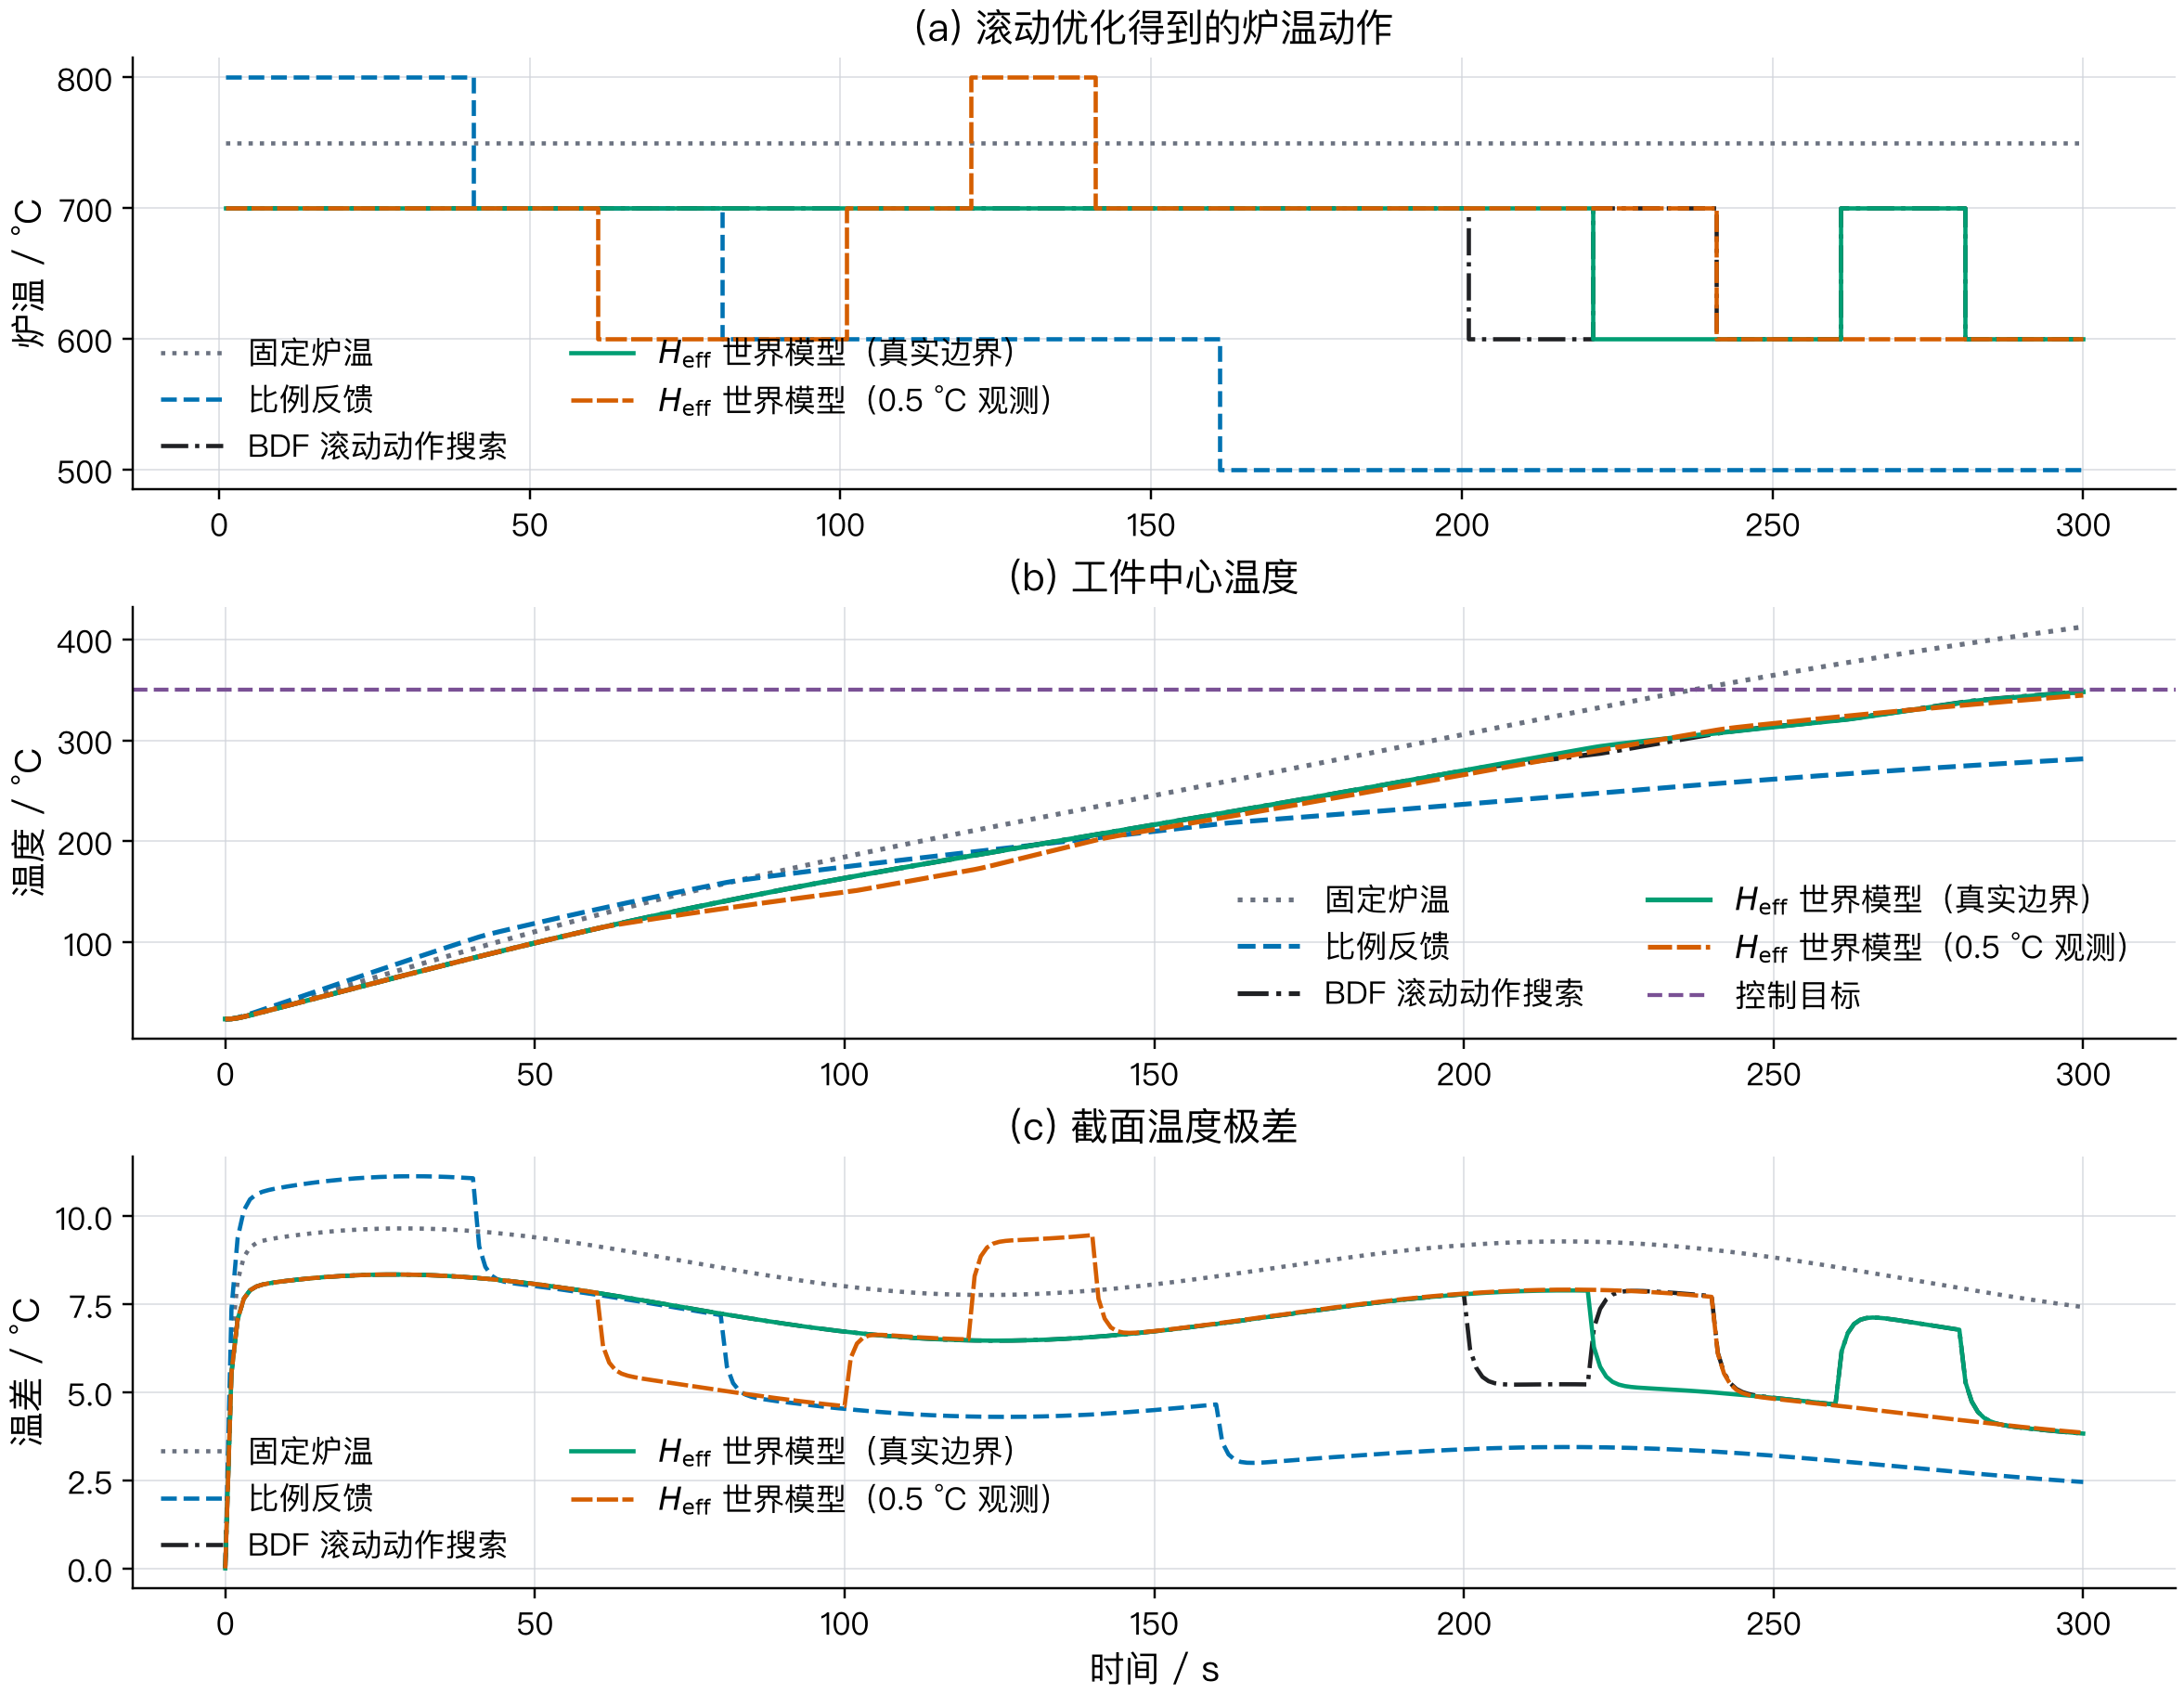
\includegraphics[width=0.96\textwidth]{closed_loop_trajectory_zh.png}
  \caption{动态边界 BDF 环境中的代表性滚动控制轨迹}
  \label{fig:closed_loop_trajectory}
\end{figure}

在相同的 10 条 ID 场景中引入五点测温，并比较四种信息条件，三个模型共形成 120 个 BDF 回合。后验均值控制的终点误差为 \SI{1.284}{\degreeCelsius}，综合目标为 16.227；风险分位控制的对应值为 \SI{1.244}{\degreeCelsius} 和 16.124。两者均为30/30个成功回合、10/10个场景全成功，95\% Wilson 区间均为 $[72.2\%,100\%]$。在这一较宽松的表面温度限制下，两种方法多次选择相同动作，尚未显示风险分位排序的明显收益。

图\ref{fig:sparse_trajectory}取模型种子 42 和联合边界轨迹 19，展示五点测量、集合状态估计和动作选择共同作用的过程。中心温度接近目标的同时，滤波器持续更新全场状态；其中的中心热电偶也持续提供对控制目标的直接测量。

\begin{figure}[H]
  \centering
  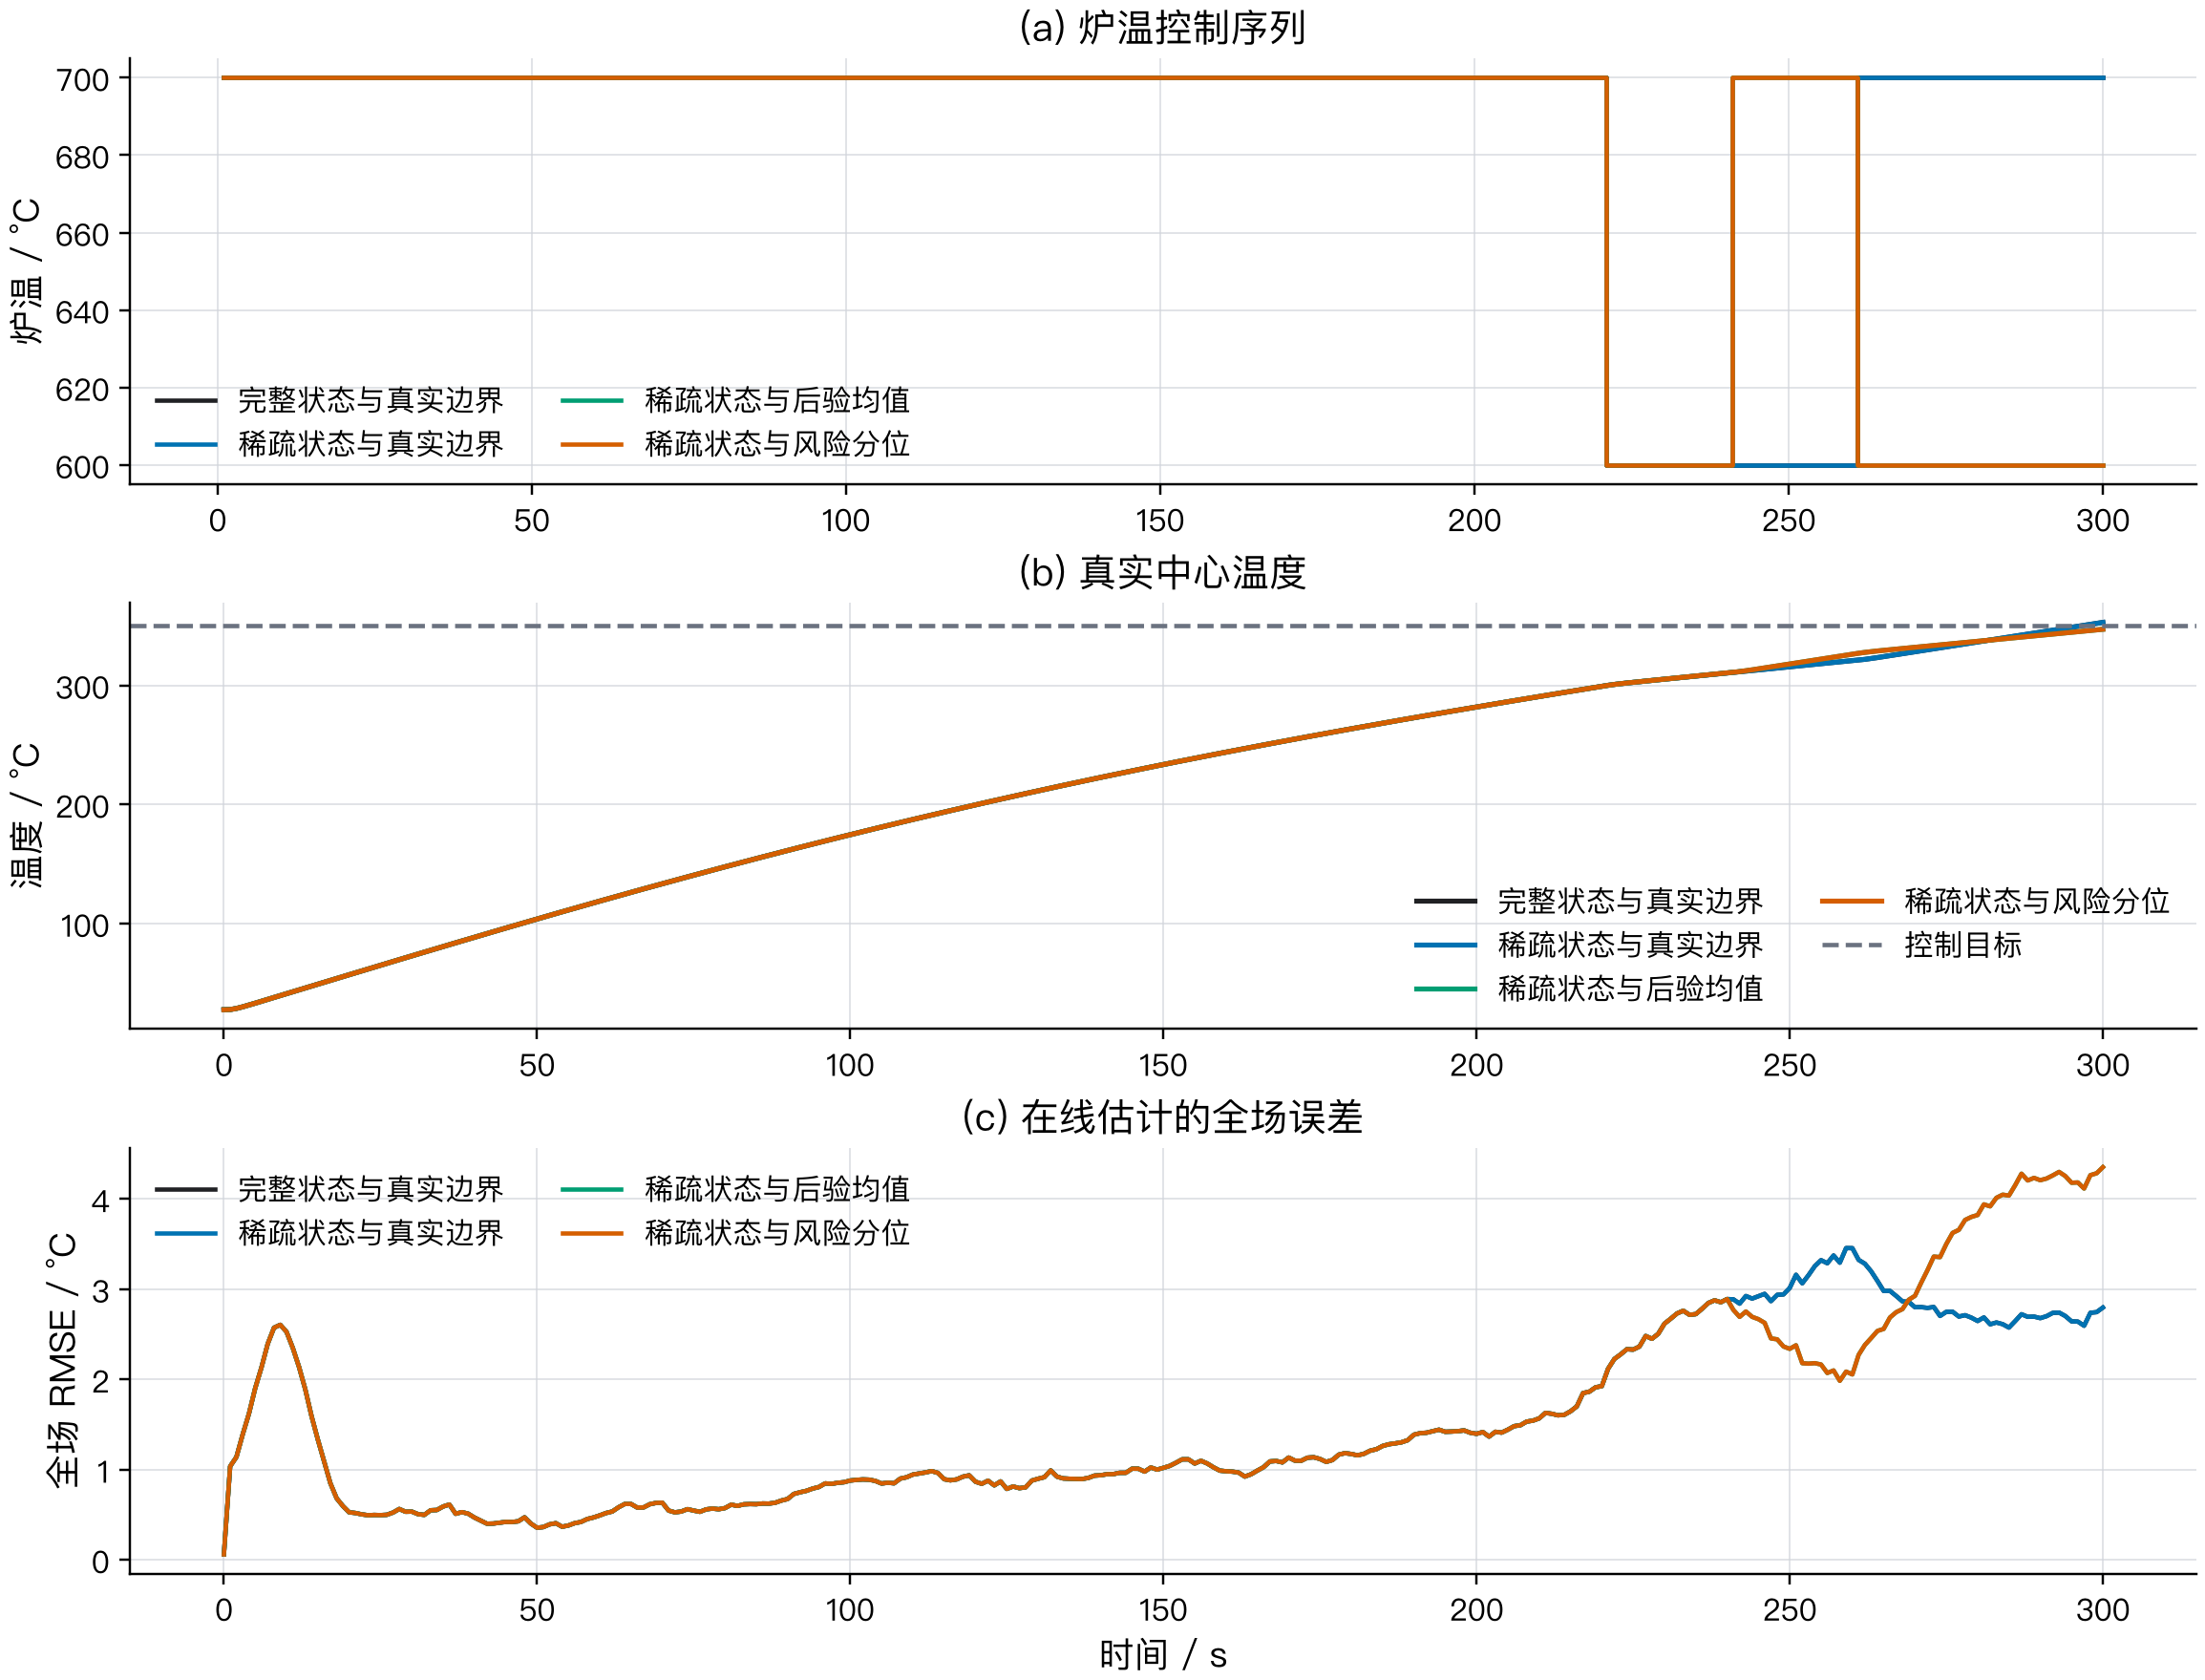
\includegraphics[width=0.96\textwidth]{sparse_observation_trajectory_zh.png}
  \caption{五点测温条件下的代表性闭环状态估计轨迹}
  \label{fig:sparse_trajectory}
\end{figure}

\subsection{删除中心测点后的配对结果}

中心测量的作用通过10条ID场景和40条独立确认参数OOD场景上的四点、五点配对实验评价，模型、滤波与控制参数保持固定。每个时刻生成五测点噪声，四点布局删除中心测量列；共同测点噪声以及滤波初始、过程噪声均相同。两种控制器、两种布局和三个模型共运行600个回合。五点分支的300个回合与对应基准的动作序列和全部非计时控制指标一致，布局比较见表\ref{tab:four_sensor_control_audit}。

\begin{table}[H]
  \centering
  \caption{四点与五点布局的闭环比较，温度指标单位：\si{\degreeCelsius}}
  \label{tab:four_sensor_control_audit}
  \small
  \resizebox{\textwidth}{!}{%
  \begin{tabular}{lcrrrcc}
    \toprule
    场景与控制器 & 测点 & 中心误差 & 平均超温 & 综合目标 & 回合成功 & 场景全成功 \\
    \midrule
    ID，后验均值 & 5 & 1.284 & 0.000 & 16.227 & 30/30 & 10/10 \\
    ID，后验均值 & 4 & 7.445 & 0.000 & 22.778 & 22/30 & 7/10 \\
    ID，风险分位 & 5 & 1.244 & 0.000 & 16.124 & 30/30 & 10/10 \\
    ID，风险分位 & 4 & 8.331 & 0.000 & 23.605 & 21/30 & 4/10 \\
    参数 OOD，后验均值 & 5 & 6.616 & 0.641 & 26.019 & 75/120 & 20/40 \\
    参数 OOD，后验均值 & 4 & 7.335 & 1.346 & 31.516 & 57/120 & 11/40 \\
    参数 OOD，风险分位 & 5 & 7.162 & 0.585 & 25.531 & 72/120 & 19/40 \\
    参数 OOD，风险分位 & 4 & 7.715 & 1.061 & 29.769 & 64/120 & 16/40 \\
    \bottomrule
  \end{tabular}}
\end{table}

在 ID 场景中，删除中心测点使后验均值控制的中心误差增加 \SI{6.161}{\degreeCelsius}，95\%配对区间为 $[4.355,8.087]$~\si{\degreeCelsius}；综合目标增加6.551，区间为 $[4.846,8.777]$。两种四点控制均未超温，主要退化表现为心部到温偏差。风险分位控制也未恢复五点条件下的跟踪精度，其场景全成功为4/10，低于后验均值控制的7/10。

在参数 OOD 确认场景中，四点后验均值控制相对五点的综合目标增加5.497，95\%区间为 $[1.483,10.368]$；回合成功比例的场景配对差为 $-15.0$ 个百分点，区间为 $[-25.8,-4.2]$ 个百分点。两种控制器的平均超温均增加，但后验均值与风险分位控制的超温配对区间分别为 $[-0.038,1.646]$ 和 $[-0.029,1.032]$~\si{\degreeCelsius}，均跨越零，不能由均值上升推定超温在总体上稳定恶化。图\ref{fig:sparse_control_audit}汇总了各工况下跟踪、超温、综合目标与成功比例的配对差。

\begin{figure}[H]
  \centering
  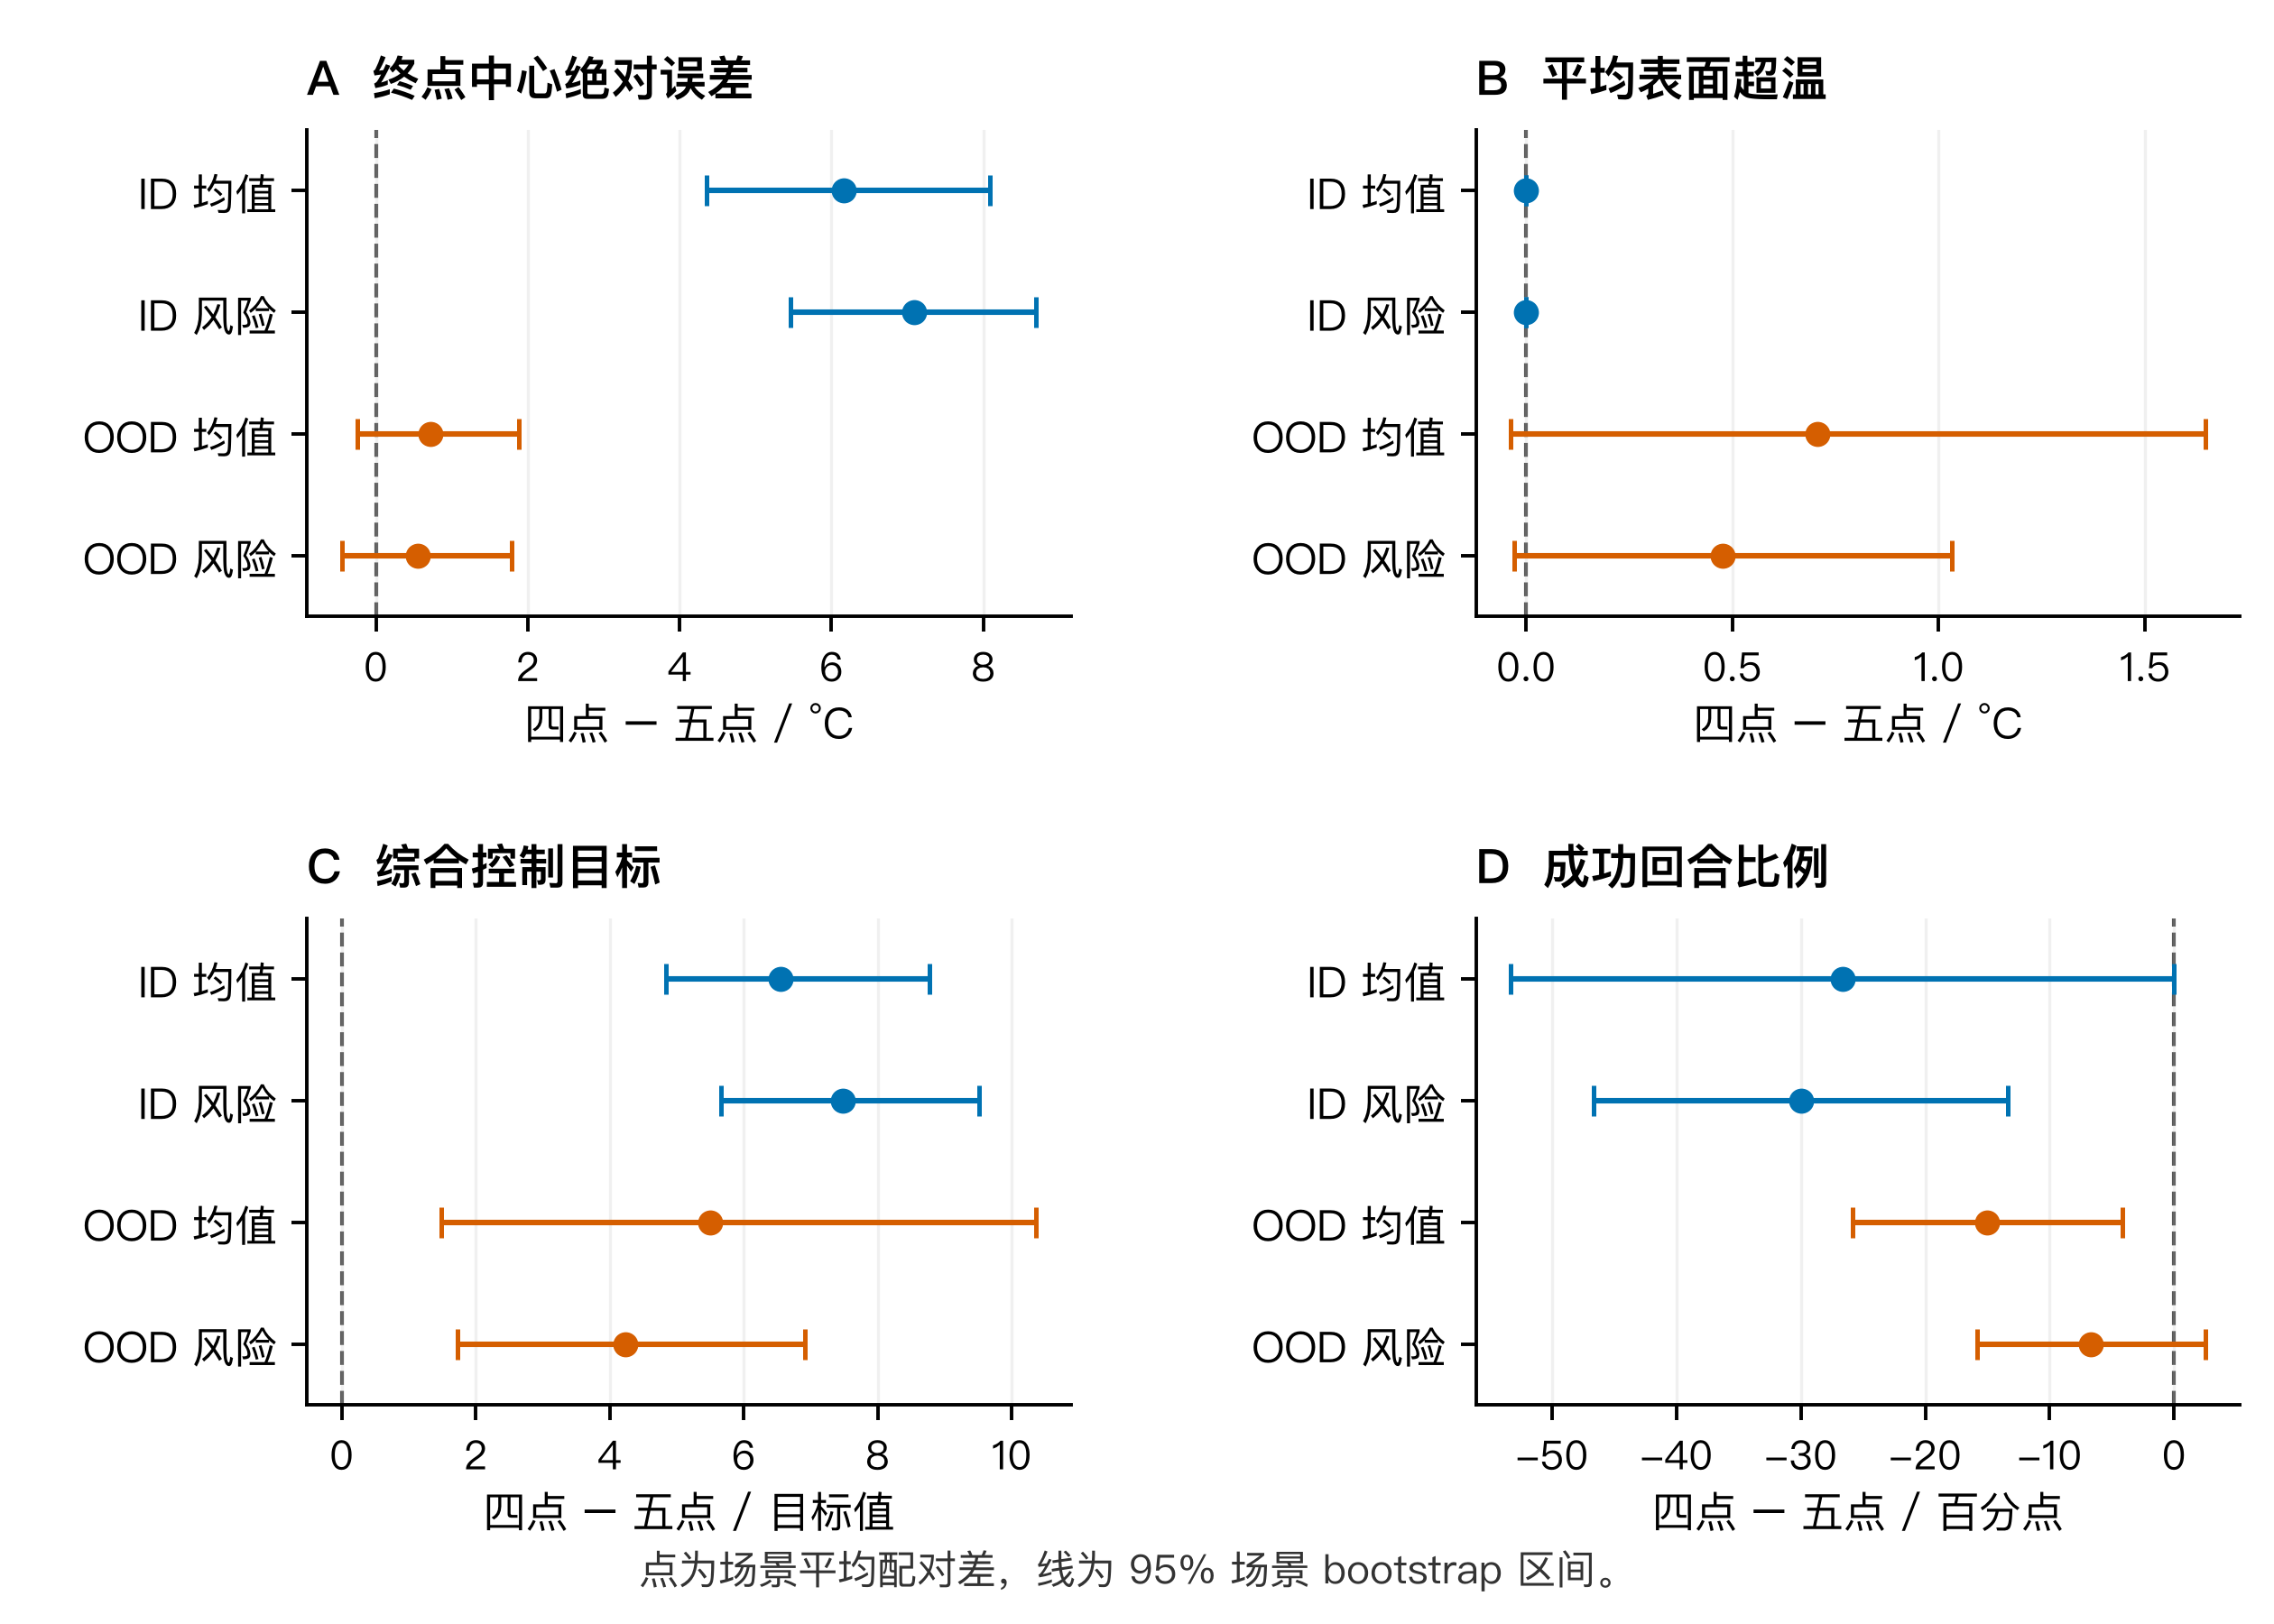
\includegraphics[width=0.98\textwidth]{sparse_control_audit.png}
  \caption{删除中心热电偶后的闭环性能变化；布局比较使用相同场景与共同随机噪声}
  \label{fig:sparse_control_audit}
\end{figure}

两种布局的闭环重建误差均在共同未观测的36个节点上计算。后验均值控制的四点、五点 RMSE 在 ID 下分别为 \SI{5.180}{\degreeCelsius}、\SI{2.216}{\degreeCelsius}，在 OOD 下分别为 \SI{7.513}{\degreeCelsius}、\SI{4.530}{\degreeCelsius}；名义90\%区间覆盖率在 ID 下为31.9\%、59.6\%，在 OOD 下为31.0\%、45.9\%。两种布局均明显欠覆盖，五点较高的控制成功比例不能作为后验区间可靠性的依据。

四点开环未测节点 RMSE 为 \SI{2.128}{\degreeCelsius} 的结果，不能直接推定相同的闭环跟踪能力或区间质量。当前方法的高 ID 成功率依赖含中心热电偶的合成观测条件；删除中心测点的退化限于本研究固定的模型、滤波和控制配置，不构成所有无中心测点方法均不可行的结论。该闭环实验使用无响应迟滞的测量，传感器响应补偿的效果仅在开环估计中得到评价。

\section{参数 OOD 下风险分位控制的证据}

风险分位控制在固定五点布局下评价，比较后验不确定性参与动作排序后的控制结果。参数 OOD 测试采用扩展边界先验，并将表面温度上限收紧为 \SI{360}{\degreeCelsius}。10条场景用于探索，互不重叠的40条场景用于独立确认探索结果；两阶段均保持后验均值与风险分位控制的配置不变。

探索集上四种控制器的结果见表\ref{tab:ood_control}。真实边界两行仍获得未来参数序列，后验两行则只使用当前估计。

\begin{table}[H]
  \centering
  \caption{10 条参数 OOD 探索场景的闭环结果，每种控制器 30 个回合}
  \label{tab:ood_control}
  \begin{tabular}{lcccc}
    \toprule
    控制器 & 中心误差/\si{\degreeCelsius} & 平均超温/\si{\degreeCelsius} & 综合目标 & 成功率 \\
    \midrule
    完整状态与真实边界 & 5.228 & 0.522 & 19.731 & $80\%$ \\
    稀疏状态与真实边界 & 5.119 & 0.750 & 20.665 & $80\%$ \\
    稀疏状态与后验均值 & 5.966 & 0.302 & 21.376 & $70\%$ \\
    稀疏状态与风险分位 & 5.822 & 0.181 & 19.638 & $70\%$ \\
    \bottomrule
  \end{tabular}
\end{table}

表中的80\%和70\%分别为24/30和21/30个成功回合，仅是执行记录比例。按场景全成功判据，四行依次为7/10、8/10、7/10、7/10；7/10与8/10的95\% Wilson区间分别为 $[39.7\%,89.2\%]$ 和 $[49.0\%,94.3\%]$。风险分位相对后验均值控制的场景配对差见表\ref{tab:risk_paired}。

\begin{table}[H]
  \centering
  \caption{10 条探索场景中风险分位减后验均值的配对统计}
  \label{tab:risk_paired}
  \begin{tabular}{lcccc}
    \toprule
    指标 & 后验均值控制 & 风险分位控制 & 平均配对差 & 95\% bootstrap 区间 \\
    \midrule
    综合目标 & 21.376 & 19.638 & $-1.737$ & $[-3.291,-0.226]$ \\
    平均超温/\si{\degreeCelsius} & 0.302 & 0.181 & $-0.121$ & $[-0.363,0.000]$ \\
    中心误差/\si{\degreeCelsius} & 5.966 & 5.822 & $-0.143$ & $[-0.720,0.454]$ \\
    \bottomrule
  \end{tabular}
\end{table}

综合目标在10个场景中有7个改善、1个不变、2个增加，平均配对差的区间低于零。平均超温降低40.0\%，但差异集中于一个高表面热负荷场景，其余9个场景均未超温；中心误差区间跨越零。每回合规划时间由 \SI{0.098}{\second} 增至 \SI{0.240}{\second}。探索集的综合目标下降伴随规划时间增加，且超温收益集中于少数场景；有限样本尚不足以支持风险分位控制的稳定优势。

\begin{figure}[H]
  \centering
  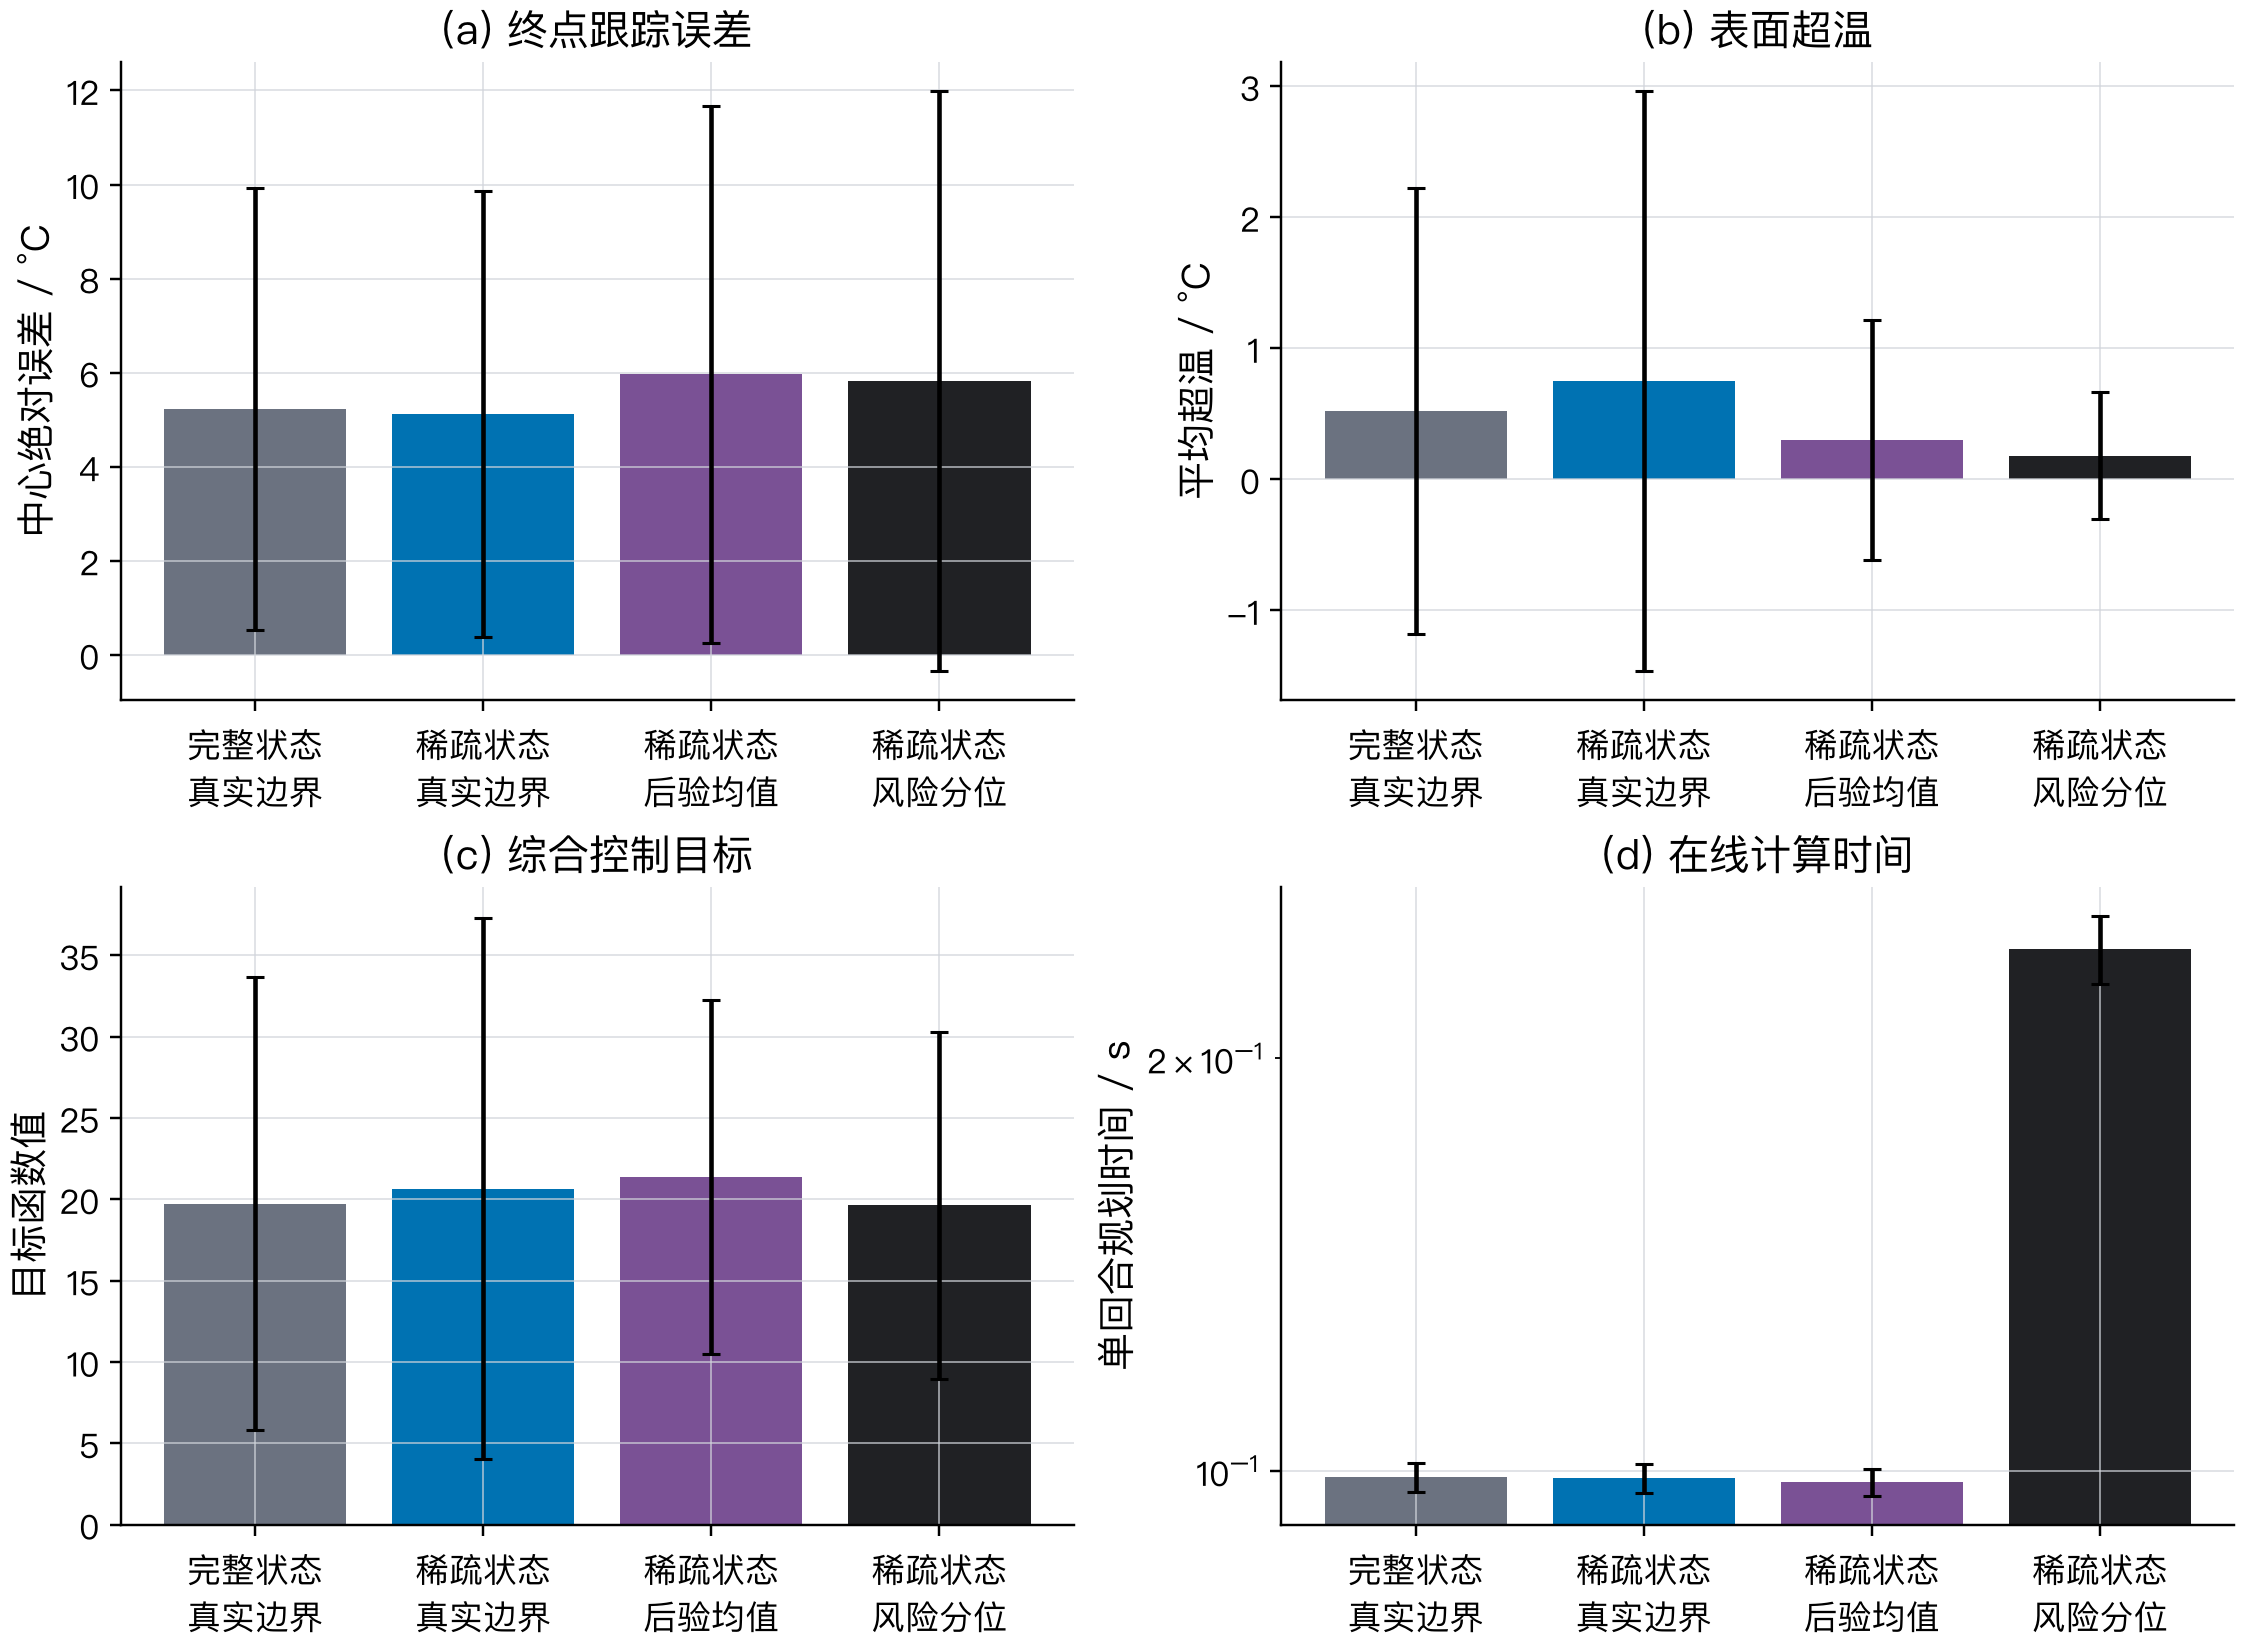
\includegraphics[width=0.96\textwidth]{ood_closed_loop_control.png}
  \caption{10 条探索场景在收紧表面温度约束后的闭环结果}
  \label{fig:ood_control}
\end{figure}

确认集从同一参数 OOD 数据池中另取40条场景，每个类别8条，排除全部探索场景。两种后验控制器各执行120个回合，以相同的场景配对口径计算结果，见表\ref{tab:risk_confirmatory}。确认集与探索集的独立性限于场景不重叠，三个训练模型仍为同一固定面板。

\begin{table}[H]
  \centering
  \caption{40 条独立确认场景中风险分位减后验均值的配对统计}
  \label{tab:risk_confirmatory}
  \resizebox{\textwidth}{!}{%
  \begin{tabular}{lcccc}
    \toprule
    指标 & 后验均值控制 & 风险分位控制 & 平均配对差 & 95\% bootstrap 区间 \\
    \midrule
    综合目标 & 26.019 & 25.531 & $-0.488$ & $[-2.802,1.950]$ \\
    平均超温/\si{\degreeCelsius} & 0.641 & 0.585 & $-0.056$ & $[-0.527,0.418]$ \\
    中心误差/\si{\degreeCelsius} & 6.616 & 7.162 & 0.546 & $[0.070,1.029]$ \\
    成功率 & $62.5\%$ & $60.0\%$ & $-2.5$ 个百分点 & $[-8.3,2.5]$ 个百分点 \\
    \bottomrule
  \end{tabular}}
\end{table}

确认集中，后验均值与风险分位控制的场景全成功数分别为20/40、19/40，95\% Wilson区间分别为 $[35.2\%,64.8\%]$、$[32.9\%,62.5\%]$；场景全成功数与表中的回合成功比例62.5\%、60.0\%对应不同统计对象。综合目标有23个场景改善、1个不变、16个增加。平均差仍偏向风险分位控制，但综合目标、超温和成功比例的95\%配对区间均跨越零；中心误差平均增加 \SI{0.546}{\degreeCelsius}，区间为 $[0.070,1.029]$~\si{\degreeCelsius}。确认结果未支持风险分位控制稳定降低综合目标或提高成功比例，并显示出中心跟踪误差增加。图\ref{fig:ood_control_extension}展示了确认集的配对差分布。

\begin{figure}[H]
  \centering
  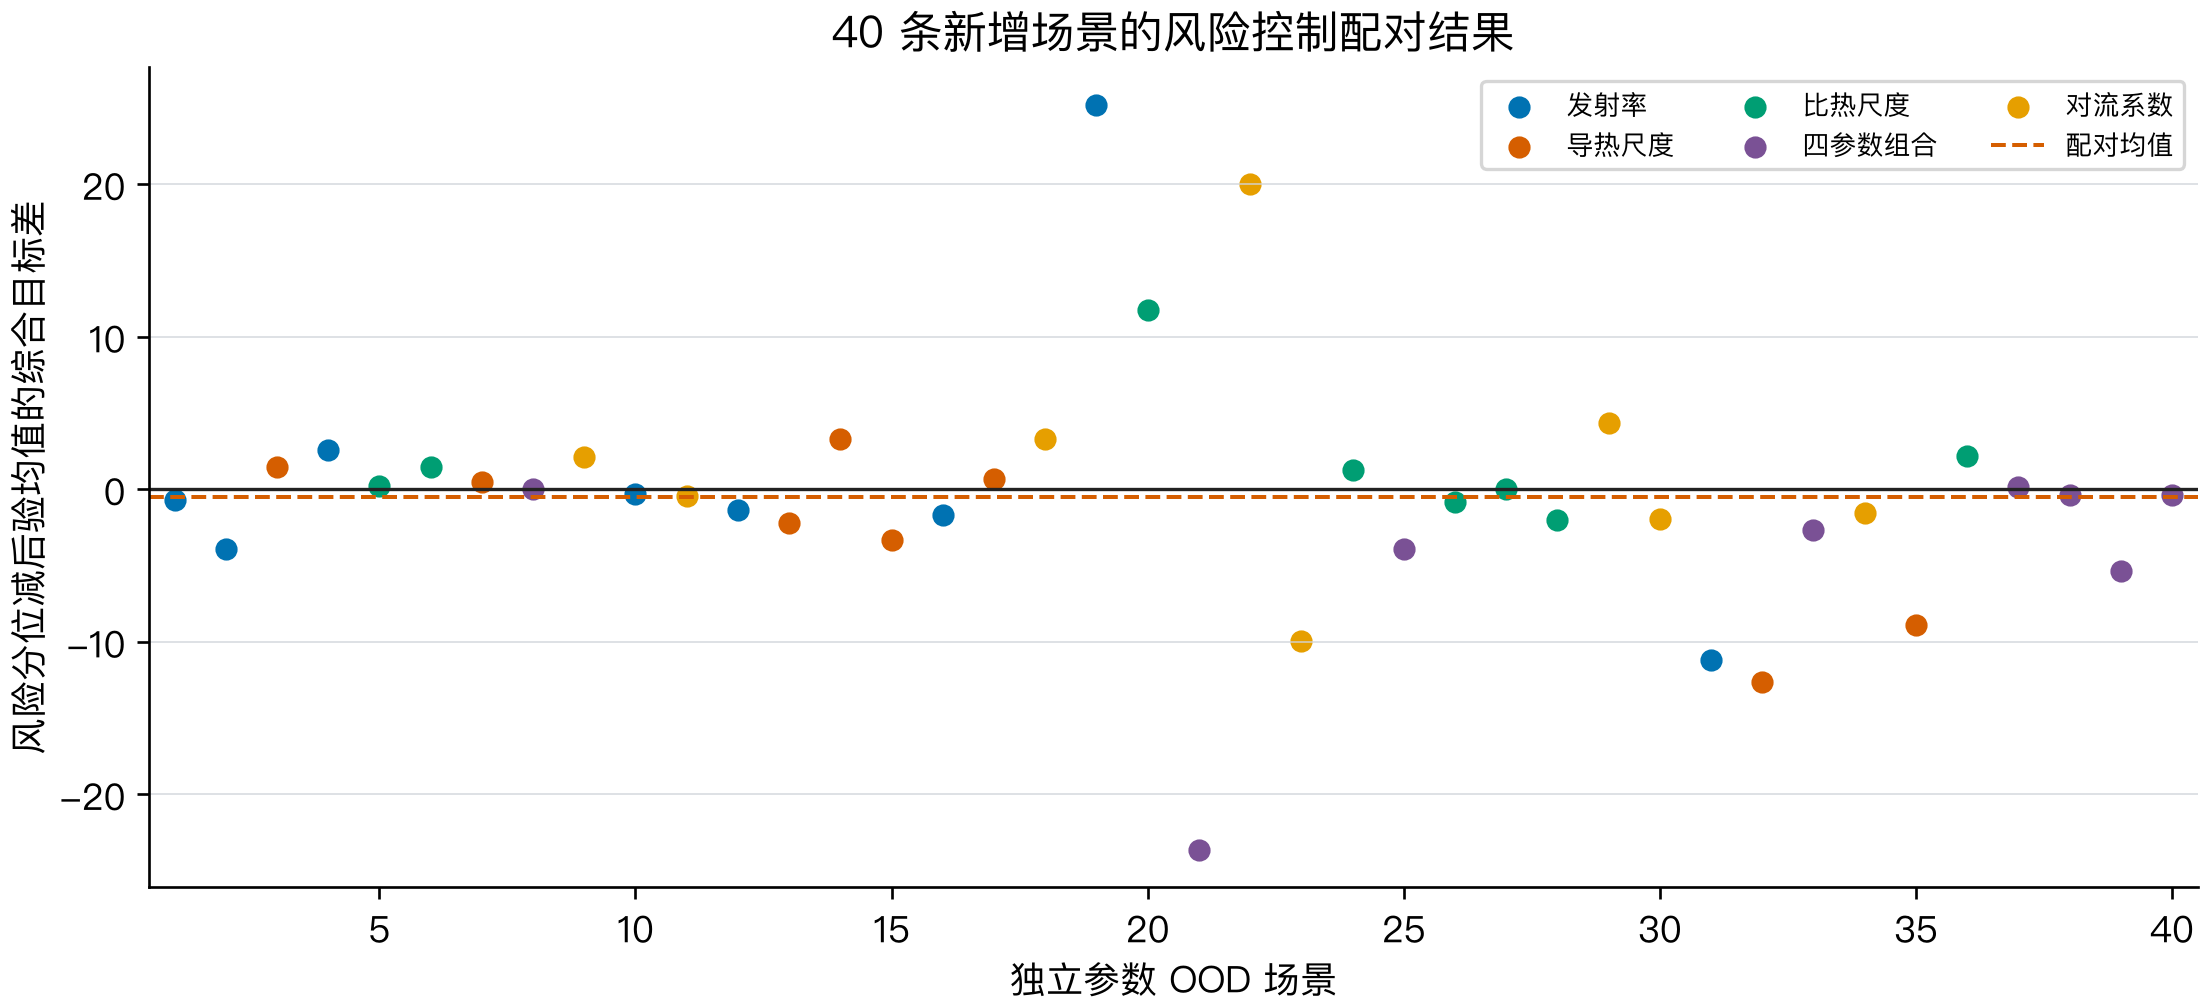
\includegraphics[width=0.94\textwidth]{ood_control_extension.png}
  \caption{40 条独立确认场景的风险控制综合目标配对差}
  \label{fig:ood_control_extension}
\end{figure}

合并两组场景作事后描述，50 条场景的综合目标配对差为 $-0.738$，95\%区间为 $[-2.630,1.248]$，仍跨越零。该合并不能替代独立确认结果，也不构成预先统一设计的50场景检验。

在本研究的数值环境和固定配置下，中心测量直接影响闭环跟踪精度，反馈轨迹上的后验区间存在欠覆盖。风险分位控制未在确认场景中表现出稳定的综合收益，四点布局下仍未达到五点布局的跟踪精度。世界模型与集合滤波构成的滚动控制器，其控制误差、成功比例及区间覆盖率均受观测条件限制。
